% Completa los datos convenientemente en las zonas marcadas con TODO

\documentclass{beamer}
%PARA VISUALIZAR PRESENTACIONN CON NOTAS USAR VISUALIZADOR "pdfpc":
%Para ver las notas, el cronometro y siguente diapo:
% pdfpc --notes=right slides.pdf
% "tecla p": para pausar el cronometro
\mode<presentation> {
  \usetheme{CambridgeUS}
  \setbeamercolor{frametitle}{fg=white,bg=blue!70}
  \setbeamercolor{block title}{fg=white,bg=blue!70}
\setbeamercolor{block body}{fg=black,bg=blue!10}
  \usecolortheme{seahorse} % color naranja
}
\setbeamercolor{titlelike}{fg=white,bg=blue!70}  % Cambia el color de la caja del título de la página inicial

\setbeamertemplate{navigation symbols}{} % ocultar iconos de navegación
\setbeamerfont{subsection in toc}{size=\small} % reducir tamaño en TOC
\setbeamerfont{date}{size=\tiny}
\usepackage[spanish]{babel}
\usepackage[utf8]{inputenc}
\usepackage{graphicx}
\usepackage{booktabs}
\usepackage{hyperref}
\usepackage{multicol}
\usepackage{pgfpages}
\usepackage{listings}
\usepackage{multimedia}
\usepackage[export]{adjustbox}
\usepackage{outlines} % Para poner bullets tabulados (\1 \2 \3 ...) y no items

\usepackage{array,tabularx} % para tabular leyenda de ecuaciones
\newenvironment{conditions*} % entorno de "leyenda de ecuación"
  {\par\vspace{\abovedisplayskip}\noindent
   \tabularx{\columnwidth}{>{$}l<{$} @{\ : } >{\raggedright\arraybackslash}X}}
  {\endtabularx\par\vspace{\belowdisplayskip}}
  
% USO DE NOTAS
% \setbeameroption{hide notes} % Para mostrar u ocultar (hide/show)
% \setbeameroption{show only notes} % Mostrar solo las notas
\setbeameroption{show notes on second screen=right} % Mostrar notas en otra pantalla
\setbeamertemplate{note page}{ % asi solo muestro el texto de las notas
  \insertnote%
}

%========= TODO: datos internos del documento
\hypersetup{
	pdftitle={Defensa de trabajo de fin de grado de Elisa Jazmín Matos Juárez},
	pdfauthor={Elisa Jazmín Matos Juárez},
	pdfsubject={Robot asistencial doméstico low-cost con interfaz amigable para personas  mayores},
	pdfkeywords={teaching, robotics, vision, sensors, actuators, raspberry},
	pdfproducer={pdfLaTeX},
  colorlinks=true,
  linkcolor=blue
}
%=========

%========= TODO: diapositiva de portada
\title[Robot asistencial doméstico]{Robot asistencial doméstico low-cost con interfaz amigable para personas  mayores} % El título reducido aparece en la parte inferior de todas las diapositivas
                                         % El título completo aparece solo en la diapositiva de portada
\author[Elisa Jazmín Matos Juárez]{Elisa Jazmín Matos Juárez}
\institute[URJC]
{
\textit{\href{ej.matos.2020@alumnos.urjc.es}{\color{blue}
{\underline{ej.matos.2020@alumnos.urjc.es}}}}\\
\vspace{0.5cm}

\includegraphics[width=3cm]{figs/logo-urjc}\\
\vspace{1cm}
Trabajo Fin de Grado
}
\date{16 de julio de 2026}
%=========

%========= COMIENZO DEL DOCUMENTO
\begin{document}

%========= Portada inicial con notas
\begin{frame}[plain] % plain: quita header y footer
\large{\titlepage}
\note[item]{En esta presentación voy a hablar sobre mi trabajo}
\end{frame}

%========= Licencia
\begin{frame}
\input{licencia.tex}
\end{frame}

%========= Índice o tabla de contenidos (TOC)
\begin{frame}
\frametitle{Contenidos}
%\begin{multicols}{2} % si tengo muchas secciones, lo parte en dos columnas
  \tableofcontents[hideallsubsections] % no muestra subsecciones
%\end{multicols}
\note[item]{La presentaci\'on esta dividida en 8 partes.}
\note[item]{Contexto enmarcado el proyecto}
\note[item]{Objetivos y requisitos establecidos}
\note[item]{Plataforma de desarrollo tanto Hardware como software}
\note[item]{Arquitectura del trabajo, tanto stf como hadw}
\note[item]{Experimentos realizados}
\note[item]{Conclusiones obtenidas}

\end{frame}

%========= Diapositiva "vacía" de comienzo de sección:
\section*{}
\begin{frame}{}
  \centering \Huge
  \emph{Introducción}
\note[item]{Comencemos con la introducción.}
\note[item]{Robot asistencial}
\note[item]{Interfaz amigable y sencilla}
\end{frame}

\section{Introducción}

% \subsection{Contexto general}
%========= Diapositiva con imágenes:


\begin{frame}
\frametitle{Robótica de servicio}
\begin{figure}
\begin{table}[htbp]
	\centering
	\begin{tabular}{cc}
		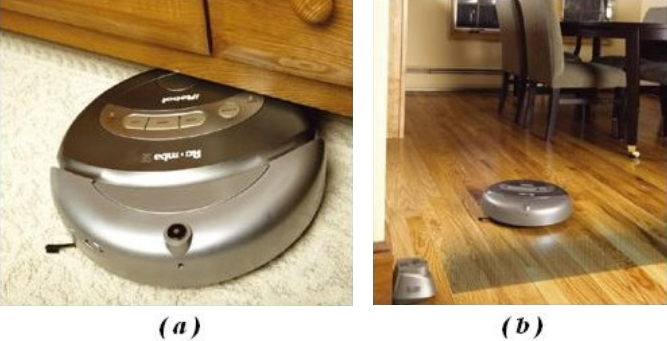
\includegraphics[width=0.3\textwidth, valign=m]{figs/roomba} & 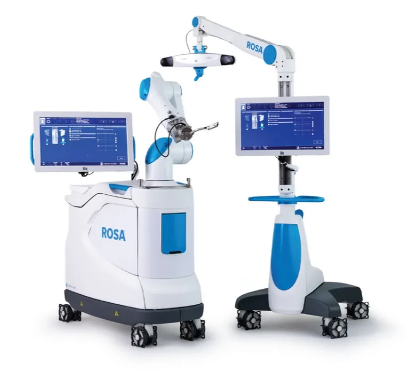
\includegraphics[width=0.3\textwidth, valign=m]{figs/rosa} \\
		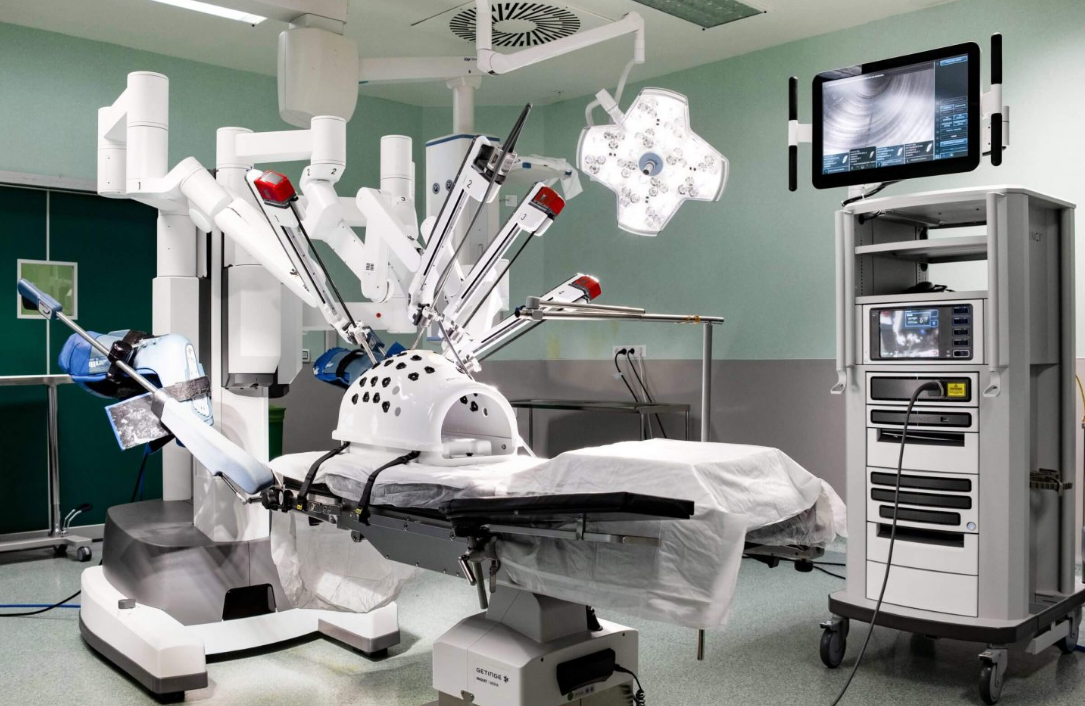
\includegraphics[width=0.3\textwidth, valign=m]{figs/Robot-Medicina} & 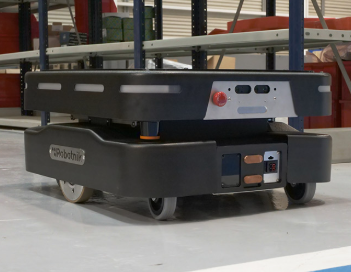
\includegraphics[width=0.3\textwidth, valign=m]{figs/log}
	\end{tabular}

\note{
    contexto del trabajo
}

\note[item]{crecimiento últimos años}
\note[item]{encontrar en hospitales, ...}
\note[item]{ayudando tareas cotidianas}

\end{table}
\end{figure}
\end{frame}


%========= Diapositiva con imágenes:
\begin{frame}
\frametitle{Robótica asistencial}
\begin{figure}
\centering
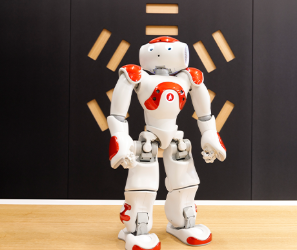
\includegraphics[height=4.5cm]{figs/nao}
\hspace{0.8cm}

\includegraphics[height=4.5cm]{figs/pepper}

\note{dentro de la robotica de servicio encontramos la r asistencial}
\note[item]{envejecimiento de la población}
\note[item]{dificultad asistencia personaliza}
\note[item]{herramienta necesaria}

\end{figure}
\end{frame}

\section*{}
\begin{frame}{}
  \centering \Huge
  \emph{Estado del arte}
\end{frame}

\section{Estado del arte}

\begin{frame}
\frametitle{Arquitectura de asistencia inteligente}
\begin{figure}
\centering
\begin{block}{Características}
\begin{itemize}

\note[item]{el trabajo responder 2 problemas principales.}
\note[item]{Multimodal: se interactua con el sistema de diferentes formas.}
\note[item]{Por voz, por gestos o mediente una interfaz gráfica.}

\item Sistema IoT.
\item Interacción multimodal.

\end{itemize}
\end{block}

\vspace{0.5cm}

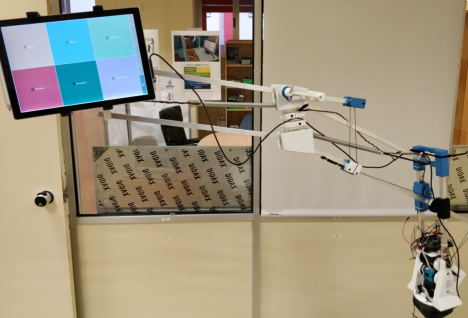
\includegraphics[height=3.6cm]{figs/assist}

\end{figure}
\end{frame}



\begin{frame}
\frametitle{EmoGame}
\begin{figure}
\centering
\begin{block}{Características}
\begin{itemize}

\note[item]{el trabajo responder 2 problemas principales.}

\item Ayuda para las personas con demencia precoz.
\item Incorpora juegos digitales.

\end{itemize}
\end{block}

\vspace{0.5cm}

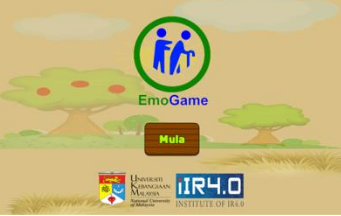
\includegraphics[height=3.6cm]{figs/emo}

\end{figure}
\end{frame}




\section*{}
\begin{frame}{}
  \centering \Huge
  \emph{Objetivos}
\note[item]{Pasemos ahora a comentar los objetivos que nos hemos propuesto con este trabajo.}
\end{frame}

\section{Objetivos}

\begin{frame}
\frametitle{Descripción del problema}
\begin{figure}
\centering
\begin{block}{Problemas}
\begin{itemize}

\note[item]{el trabajo responder 2 problemas principales.}

\item Soledad en personas mayores.
\item Escasez de personal asistencial.

\end{itemize}
\end{block}

\vspace{0.5cm}


\includegraphics[height=3.6cm]{figs/sol}
\hspace{0.4cm}
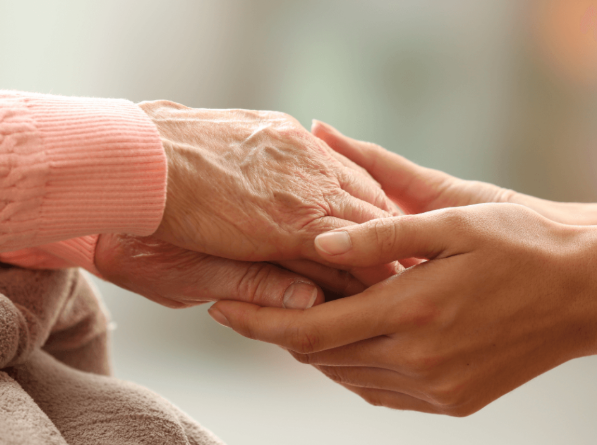
\includegraphics[height=3.6cm]{figs/mano}

\end{figure}
\end{frame}



\begin{frame}
\frametitle{Objetivos}
\begin{figure}
\centering
\begin{block}{Objetivos}
\begin{itemize}

\item Interfaz amigable y sencilla.
\item Interección personalizada.
\item Autenticación facial.
\item Uso de modelos de leguaje.

\end{itemize}
\end{block}

\vspace{0.5cm}

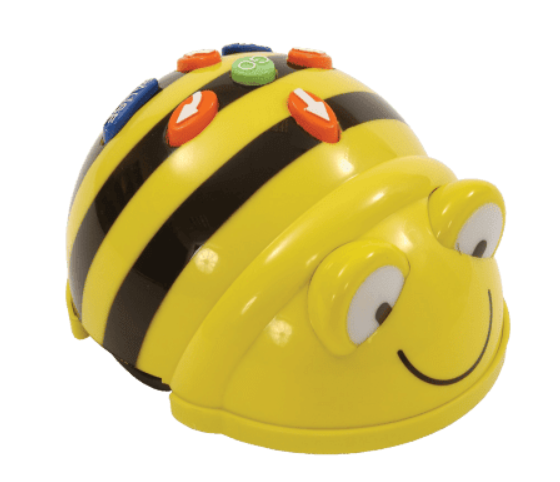
\includegraphics[height=3.6cm]{figs/bee}
\hspace{0.4cm}
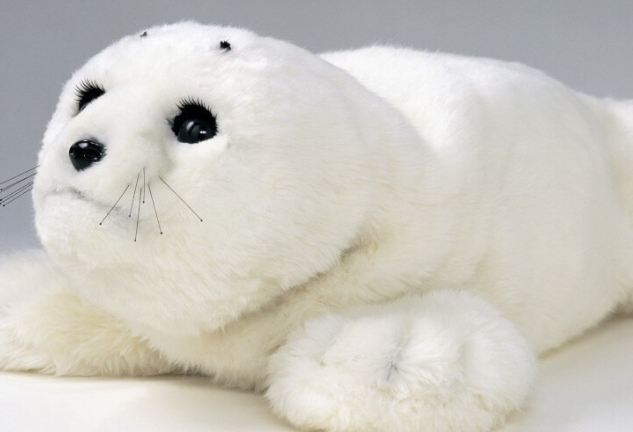
\includegraphics[height=3.6cm]{figs/nuka}

\end{figure}
\end{frame}


%========= Diapositiva con bullets en diferentes niveles (outline):
\section{Requisitos}
\begin{frame}{Requisitos}

\begin{columns}

% Columna izquierda
\begin{column}{0.55\textwidth}
\begin{outline}
\1 Bajo coste computacional.
\1 Compatibilidad con Raspberry Pi 4.
\1 Hardware low-cost.
\1 Impresión 3D.
\1 Estabilidad.
\1 Peso optimizado.
\end{outline}
\end{column}

% Columna derecha
\begin{column}{0.45\textwidth}
\centering
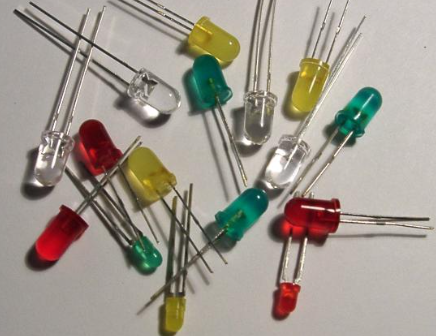
\includegraphics[width=0.47\linewidth]{figs/comp}
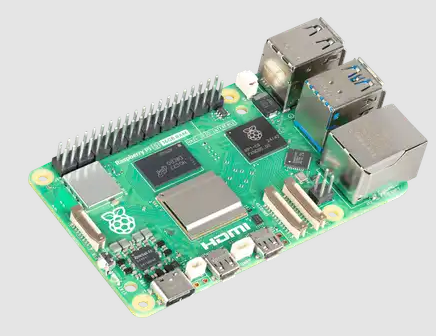
\includegraphics[width=0.47\linewidth]{figs/pi}

\vspace{0.2cm}

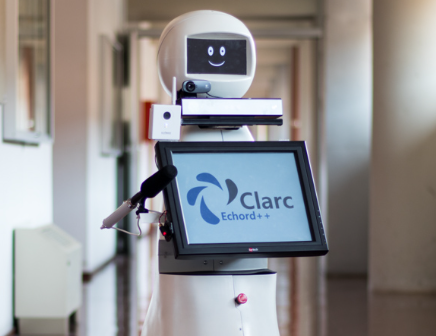
\includegraphics[width=0.47\linewidth]{figs/asis}
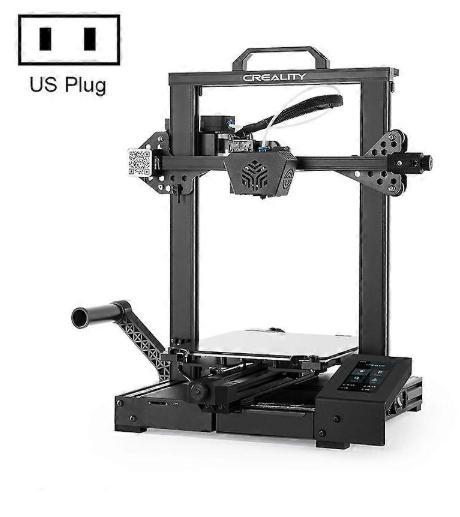
\includegraphics[width=0.47\linewidth]{figs/cre}

\end{column}

\end{columns}

\end{frame}


\begin{frame}
\frametitle{Metodología}
\begin{figure}
\centering
\begin{block}{}
\begin{itemize}

\item Desarrollo iterativo e incremental.
\item Control de versiones mediante \href{https://github.com/RoboticsURJC/tfg-ematos}{GitHub}.
\item Diario de desarrollo mediante \href{https://github.com/RoboticsURJC/tfg-ematos/wiki}{Wiki}.
\item Reuniones semanales de seguimiento.

\note[item]{Incremental: subojetivos y prueba y Validación}

\end{itemize}
\end{block}

\vspace{0.3cm}

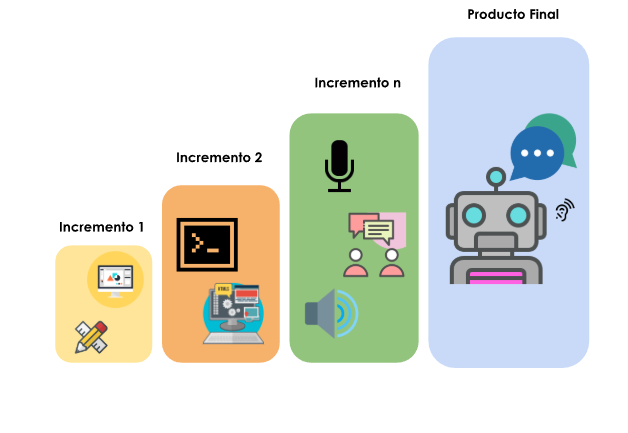
\includegraphics[height=5cm]{figs/incremento}


\end{figure}
\end{frame}


\section*{}
\begin{frame}{}
  \centering \Huge
  \emph{Plataforma de desarrollo}
\note[item]{Una vez descrito el contexto y objetivos pasemos a las plataformas de desarrollo utilizadas}
\end{frame}

\section{Plataforma de desarrollo}

\begin{frame}{Hardware}

\centering

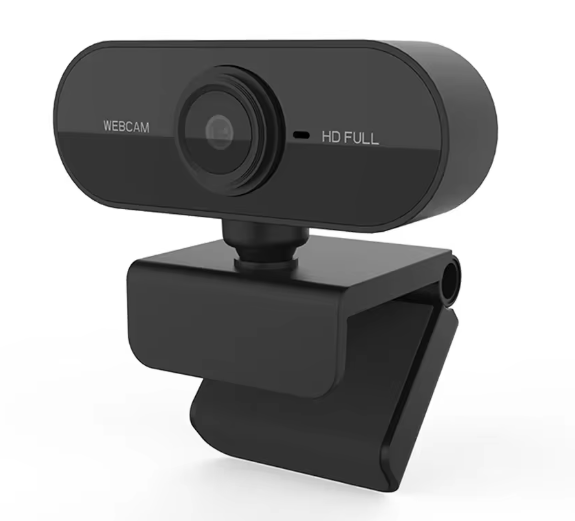
\includegraphics[width=0.25\textwidth]{figs/camara}
\hfill
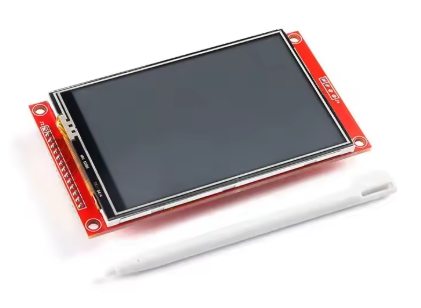
\includegraphics[width=0.25\textwidth]{figs/lcd}
\hfill
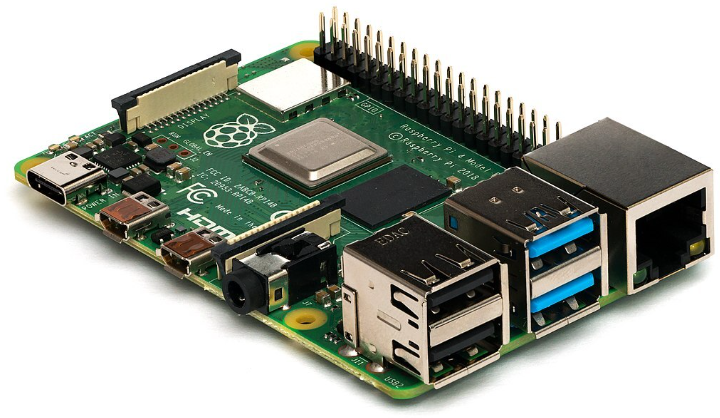
\includegraphics[width=0.25\textwidth]{figs/raspberry-pi}

\vspace{0.2cm}

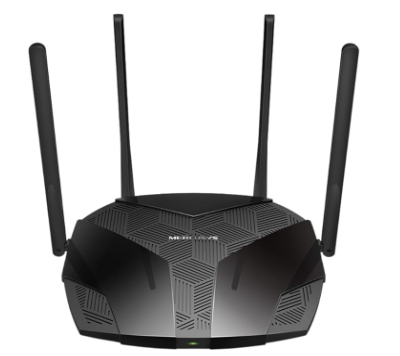
\includegraphics[width=0.25\textwidth]{figs/router}
\hfill
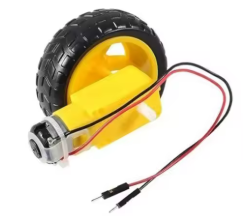
\includegraphics[width=0.25\textwidth]{figs/rueda}
\hfill
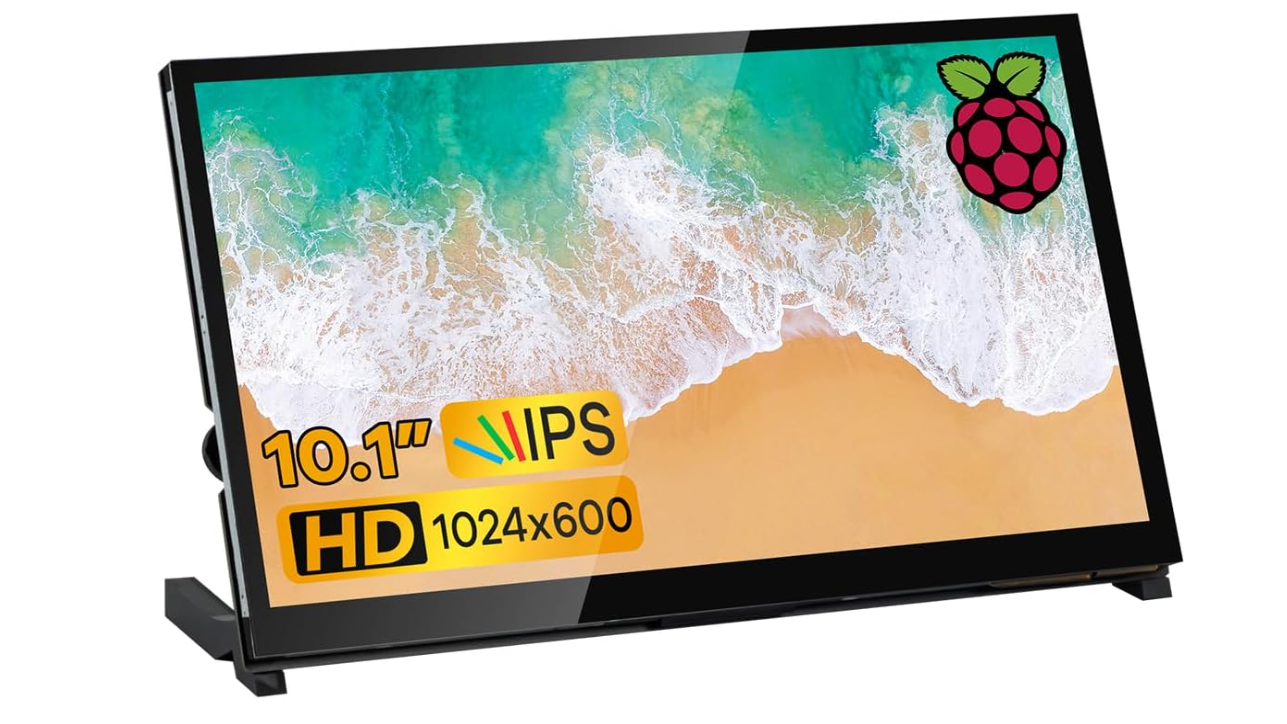
\includegraphics[width=0.25\textwidth]{figs/pantalla}

\end{frame}


\begin{frame}
\frametitle{Software}
\begin{figure}
\centering


\includegraphics[height=3cm]{figs/opencv}
\hspace{0.5cm}

\includegraphics[height=3cm]{figs/freecad}

\vspace{0.3cm}


\includegraphics[height=2.2cm]{figs/cirkit}

\end{figure}
\end{frame}


\section*{}
\begin{frame}{}
  \centering \Huge
  \emph{Arquitectura hardware del sistema}
\note[item]{Pasemos ahora a comentar los objetivos que nos hemos con este trabajo.}
\end{frame}

\section{Arquitectura hardware del sistema}

\begin{frame}
\frametitle{Estructura del robot}
\begin{figure}
\centering
\begin{block}{Características principales}
\begin{itemize}

\item Diseño modular y desmontable.
\item Peso ligero.
\item Estructura estable.

\end{itemize}
\end{block}

\vspace{0.5cm}

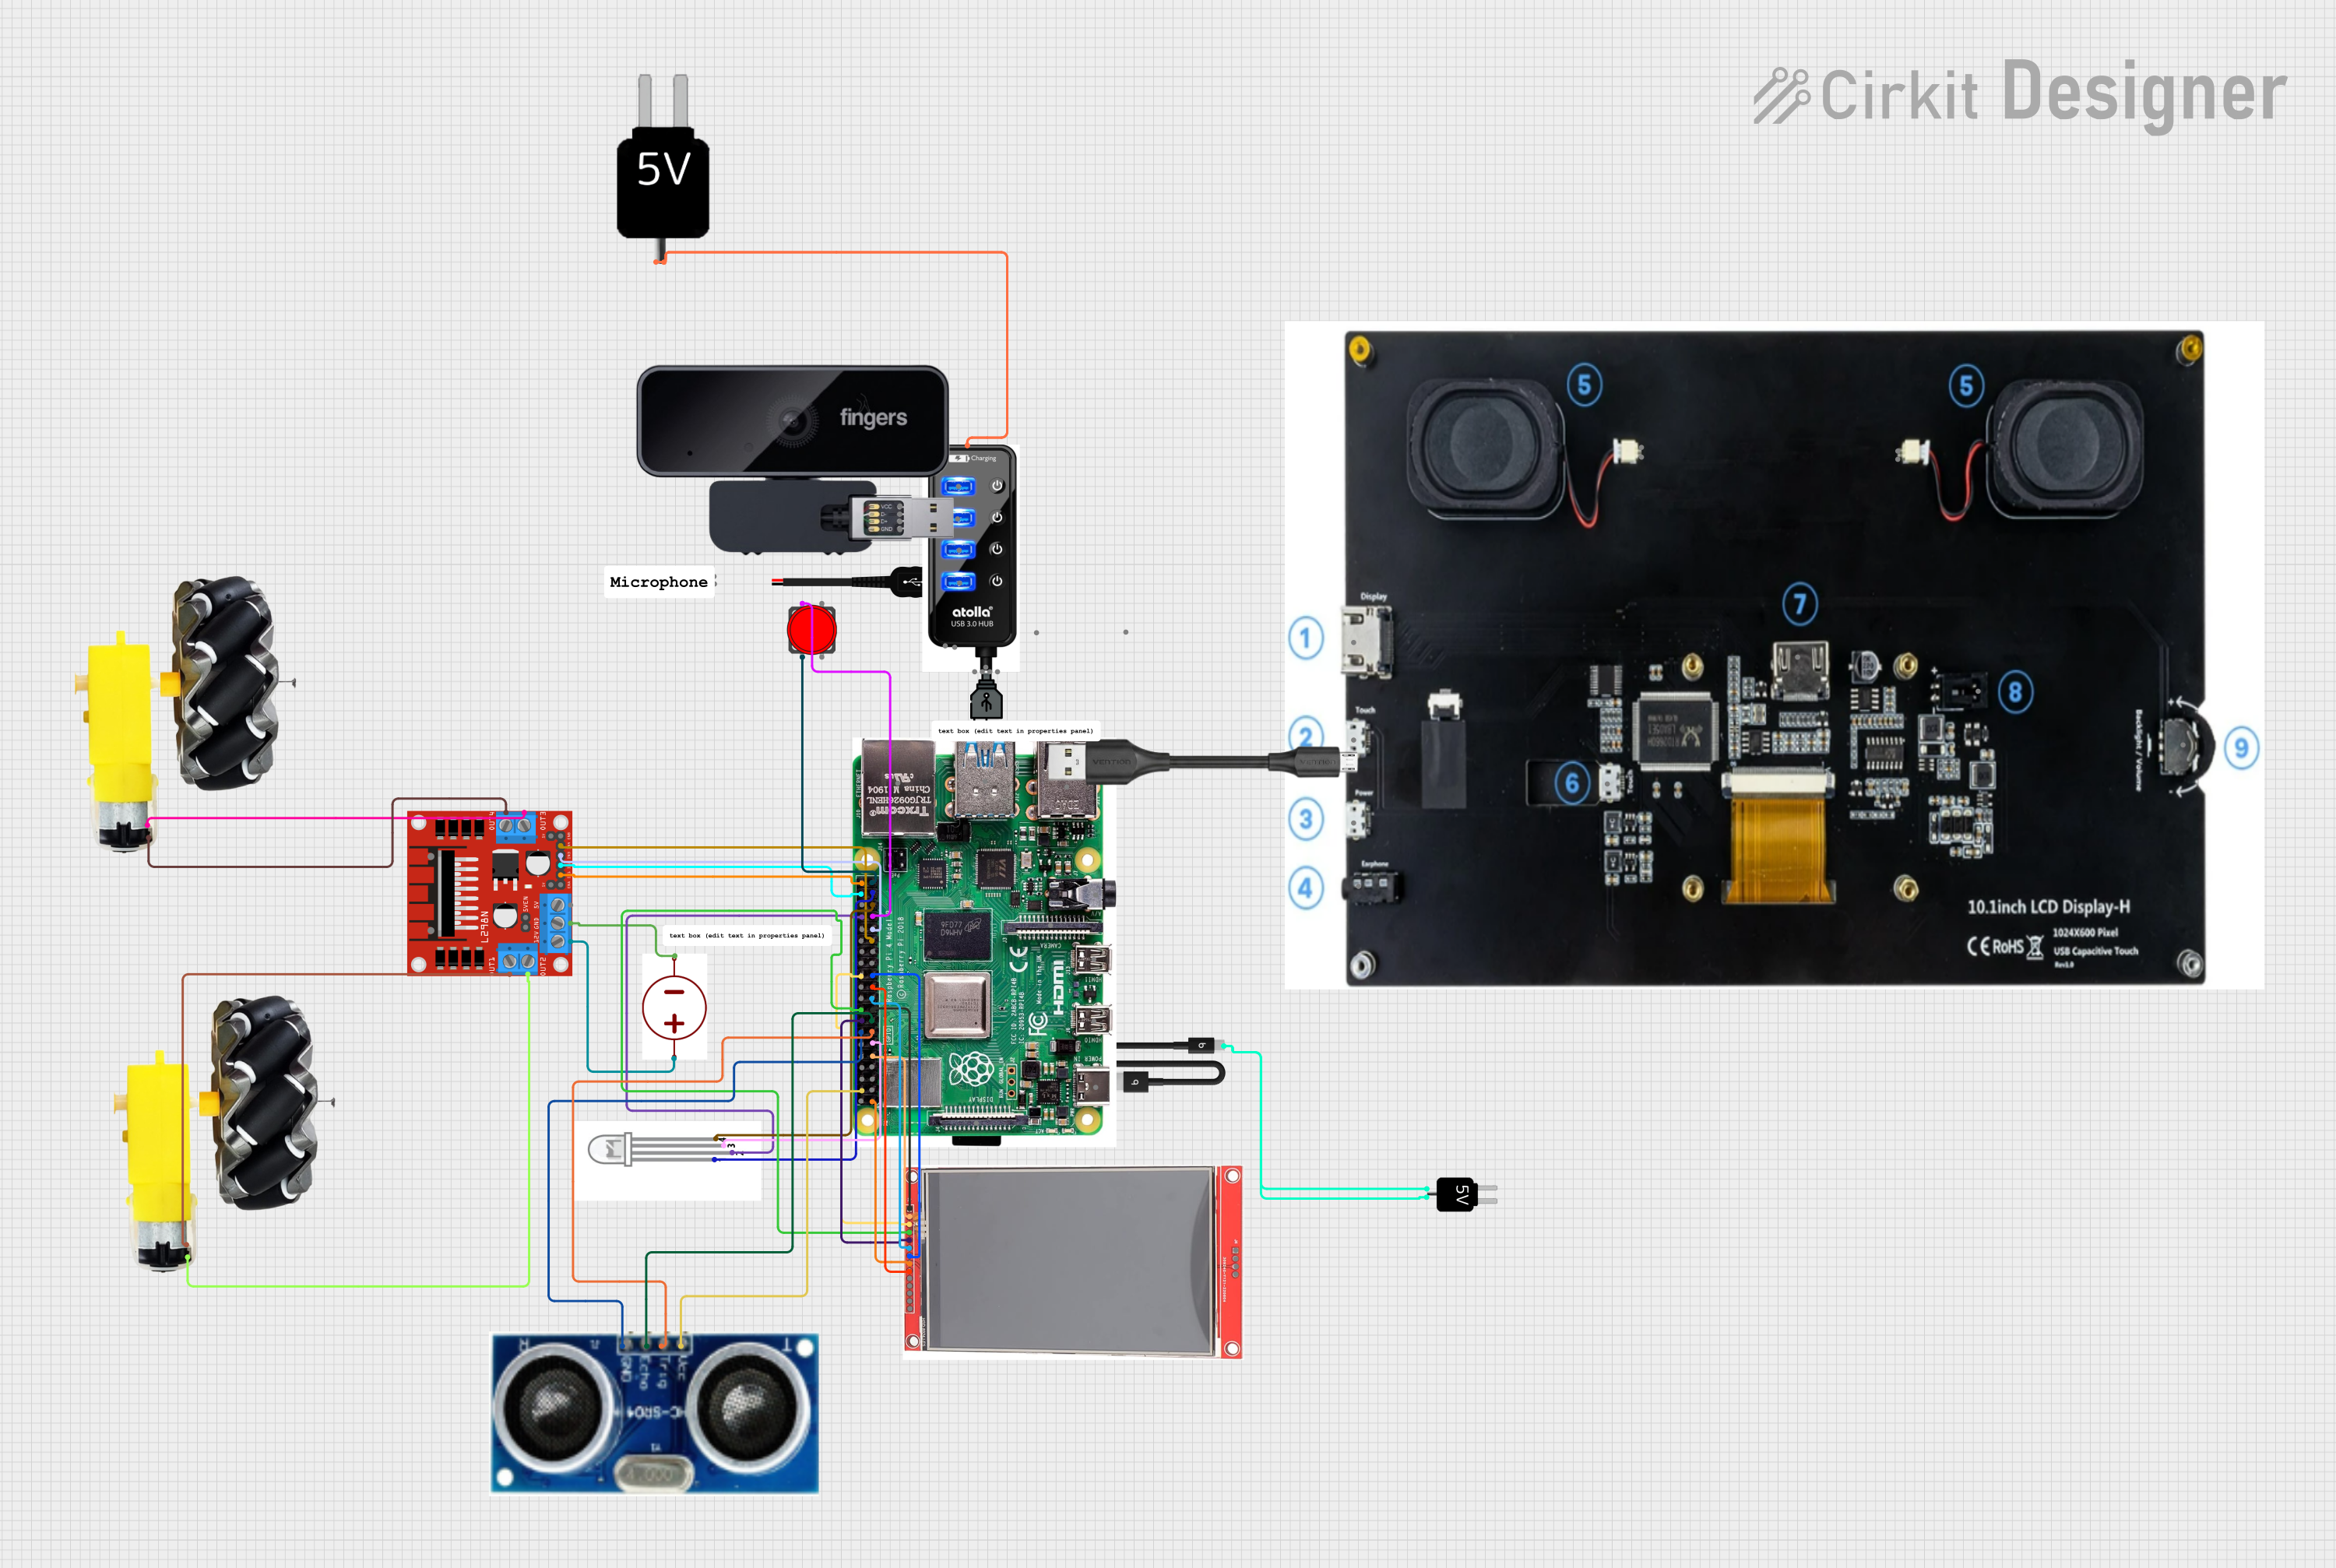
\includegraphics[height=3.6cm]{figs/circuit_image}
\hspace{0.4cm}
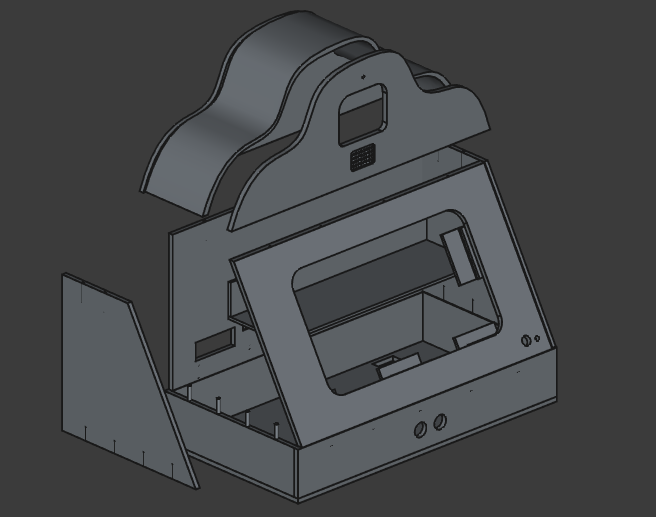
\includegraphics[height=3.6cm]{figs/3D}

\end{figure}
\end{frame}


\begin{frame}
\frametitle{Bocetos}
\begin{figure}
\centering

\vspace{0.5cm}

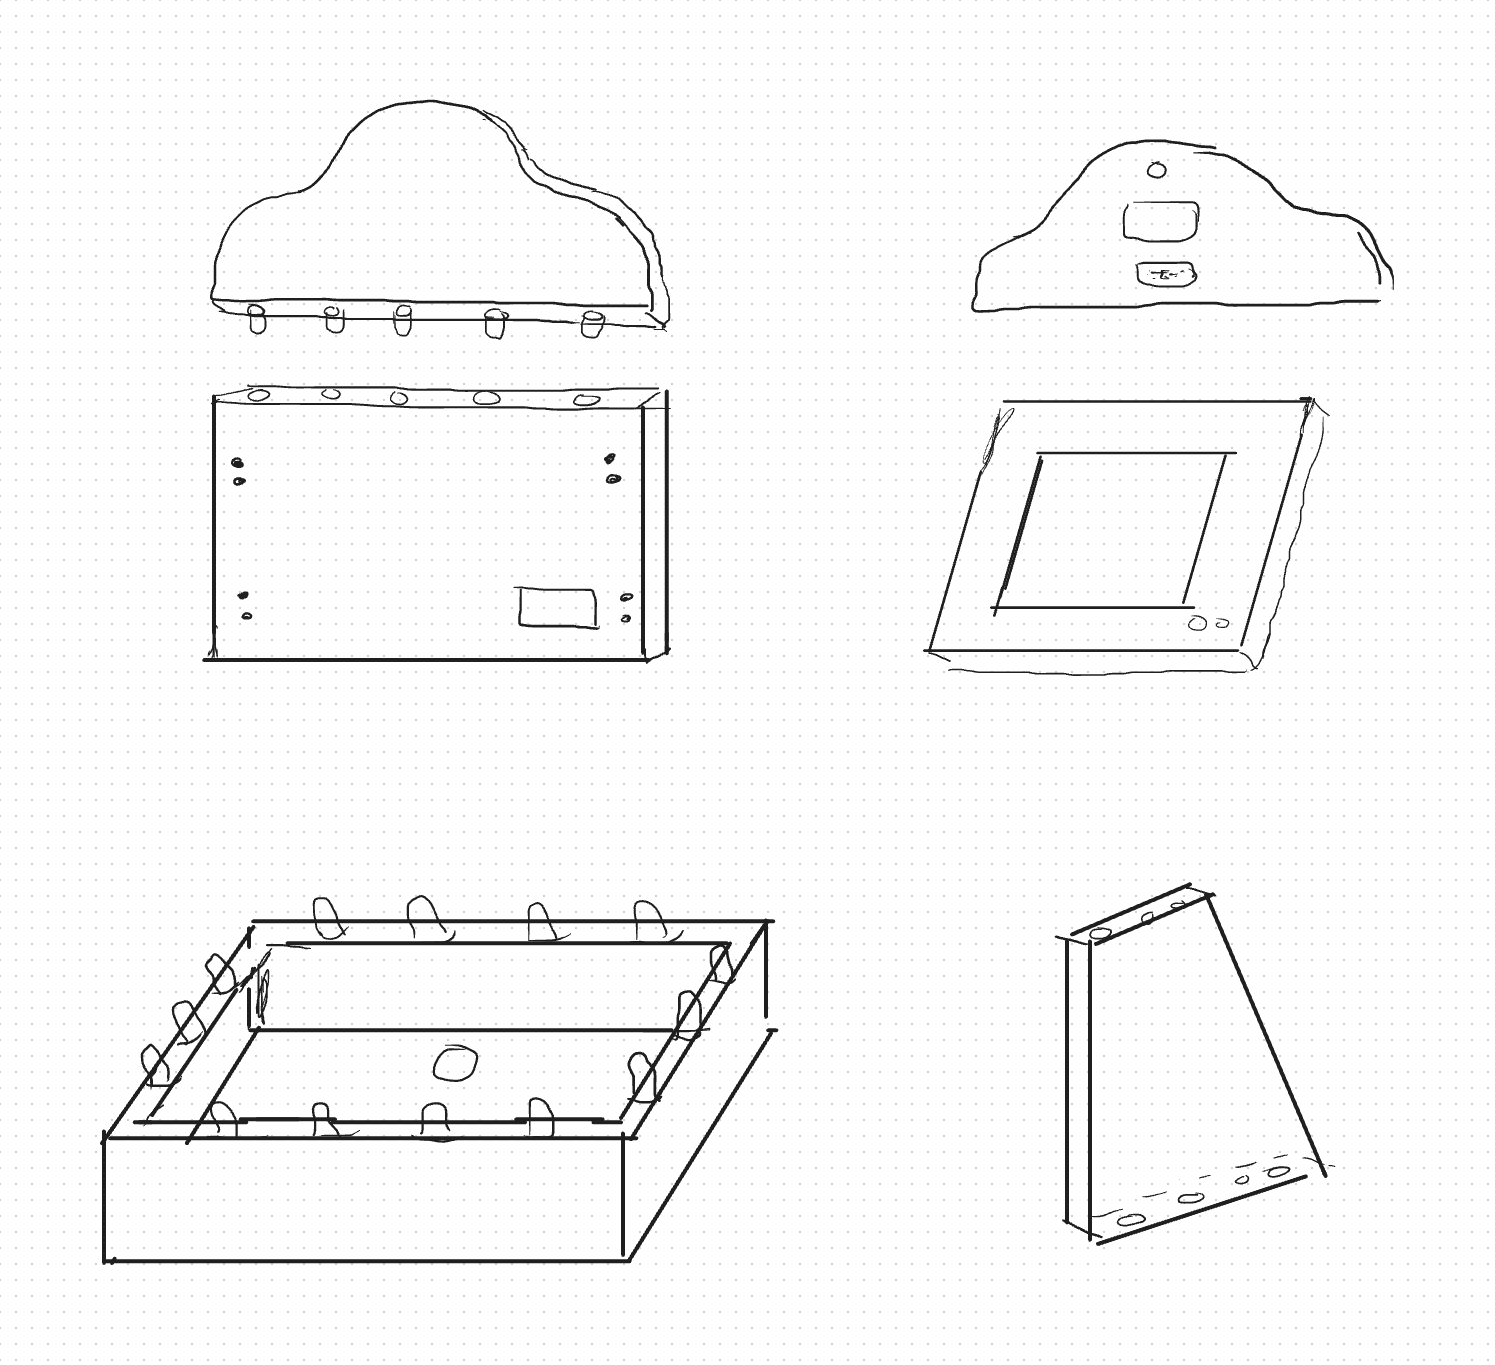
\includegraphics[height=6cm]{figs/boceto}

\end{figure}
\end{frame}


\begin{frame}
\frametitle{Prototipo}
\begin{figure}
\centering

\vspace{0.5cm}


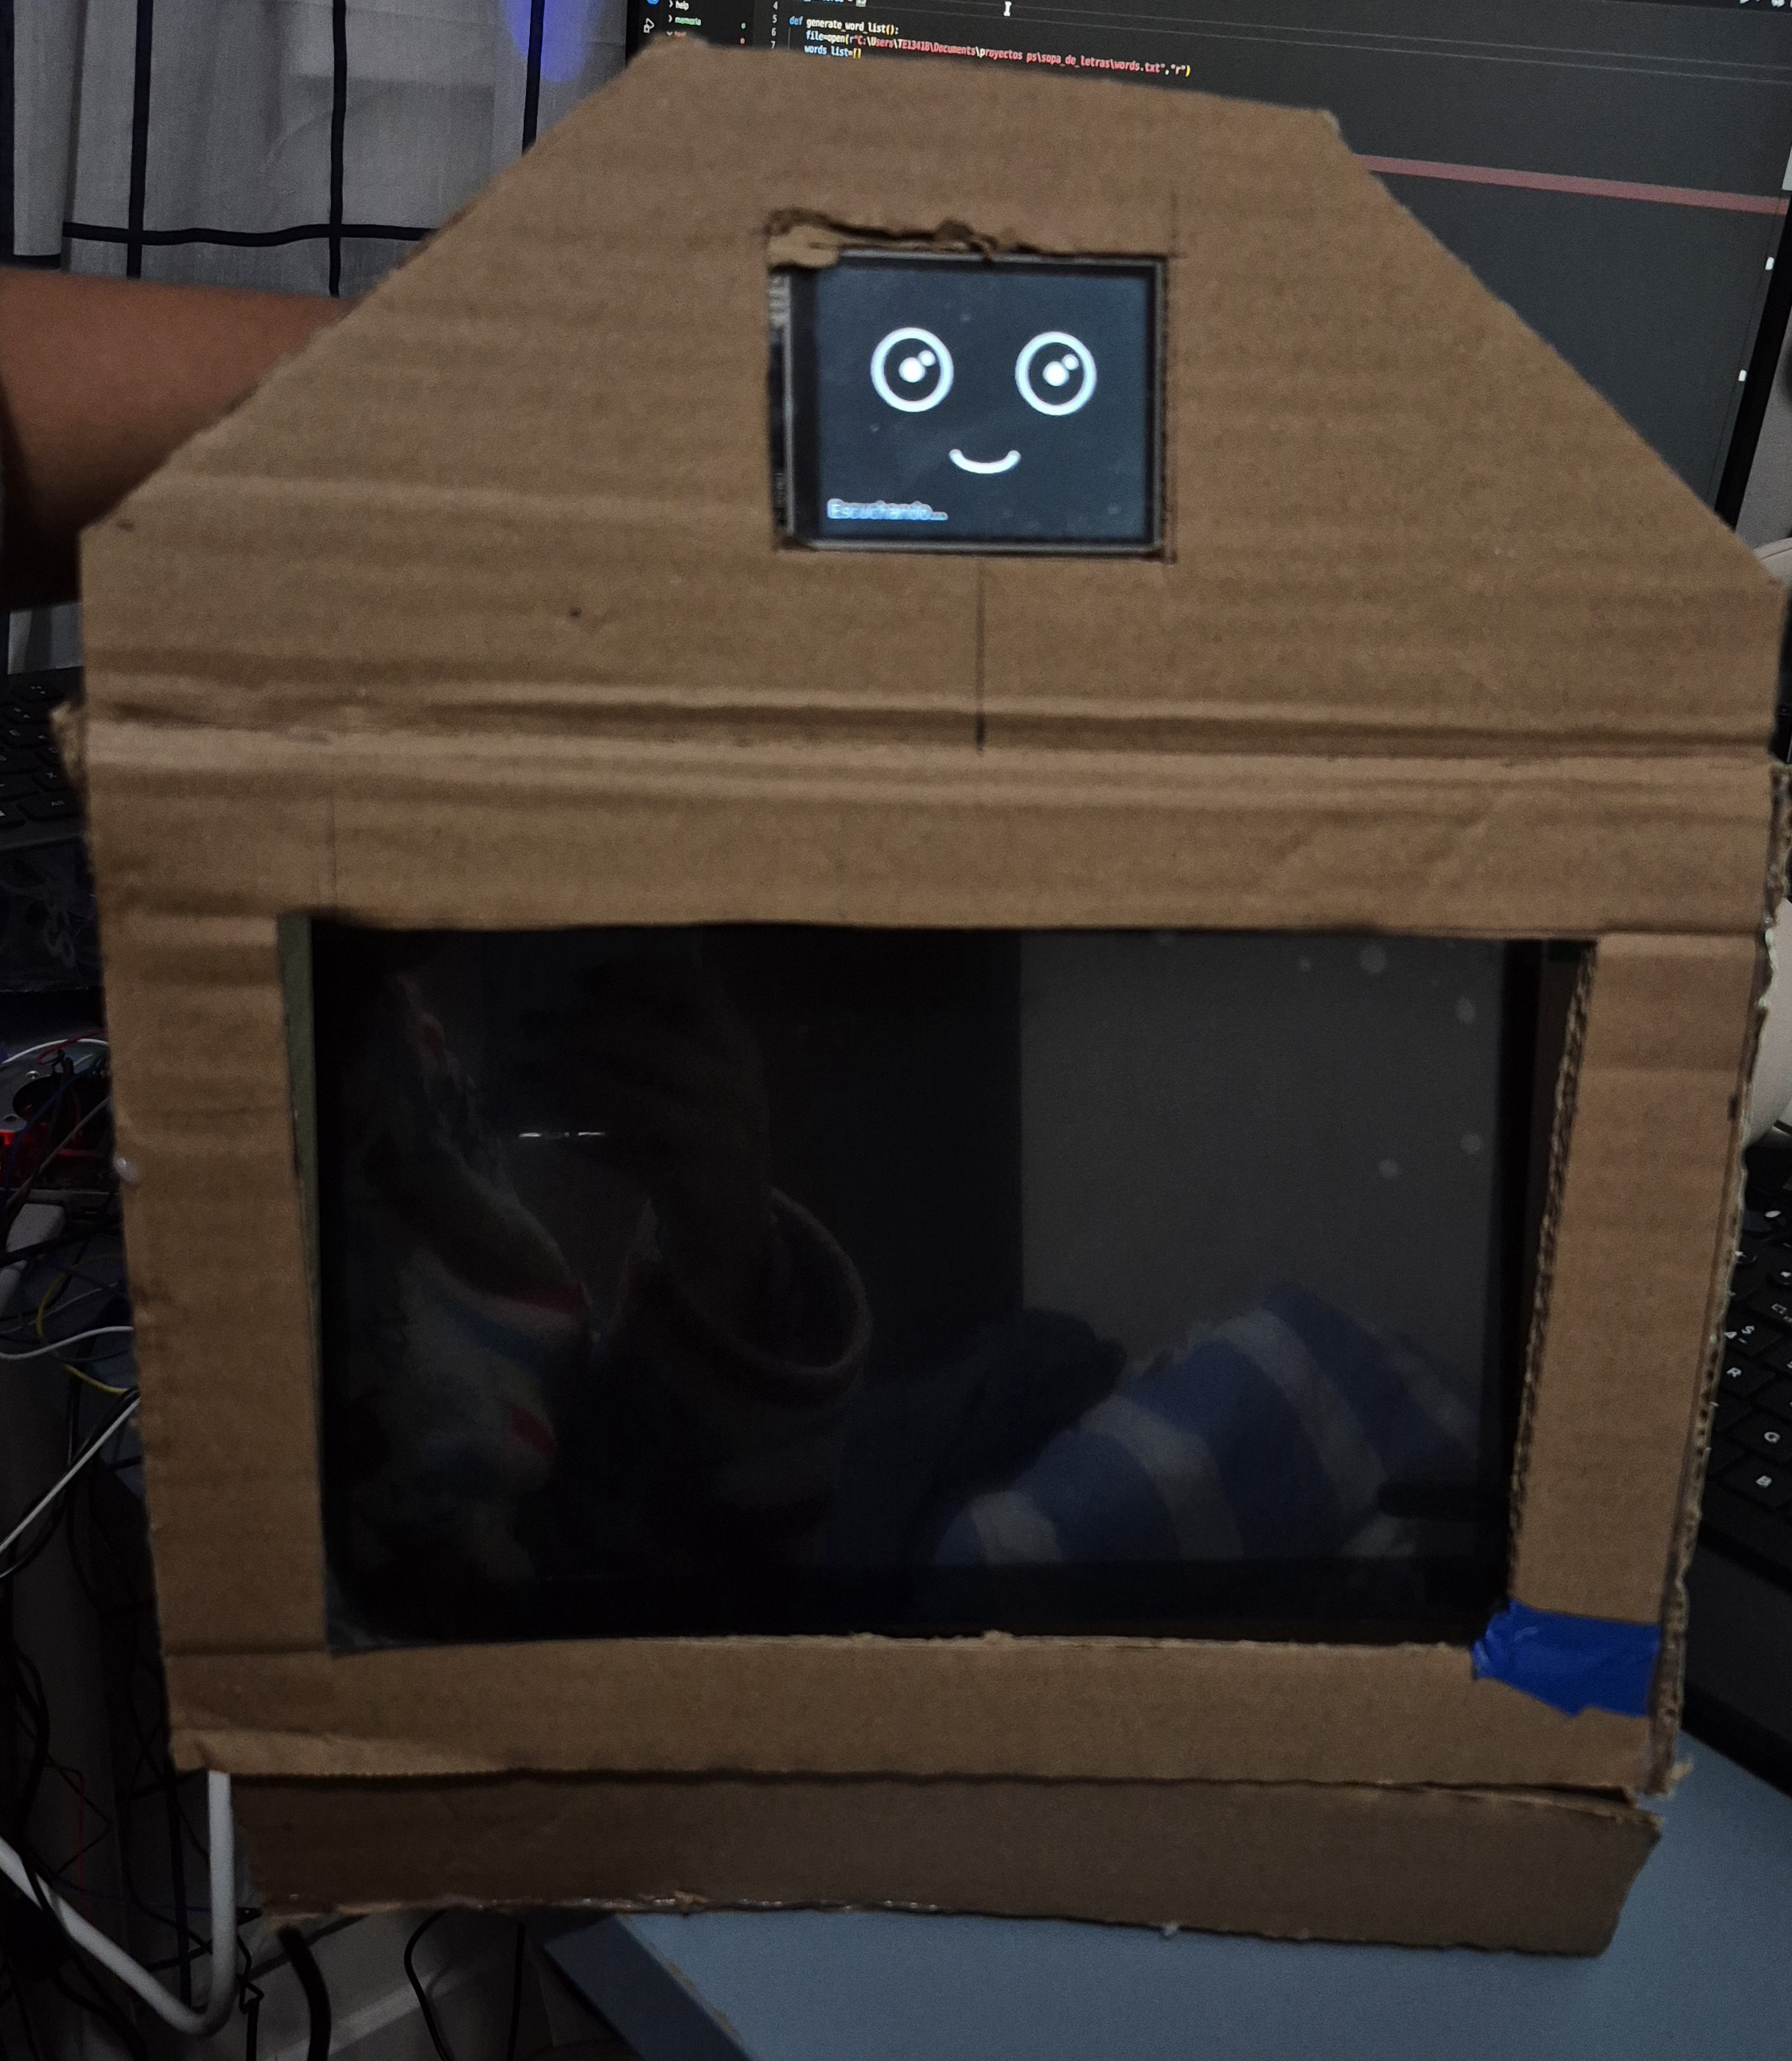
\includegraphics[height=3.6cm]{figs/modelo_carton}
\hspace{0.4cm}
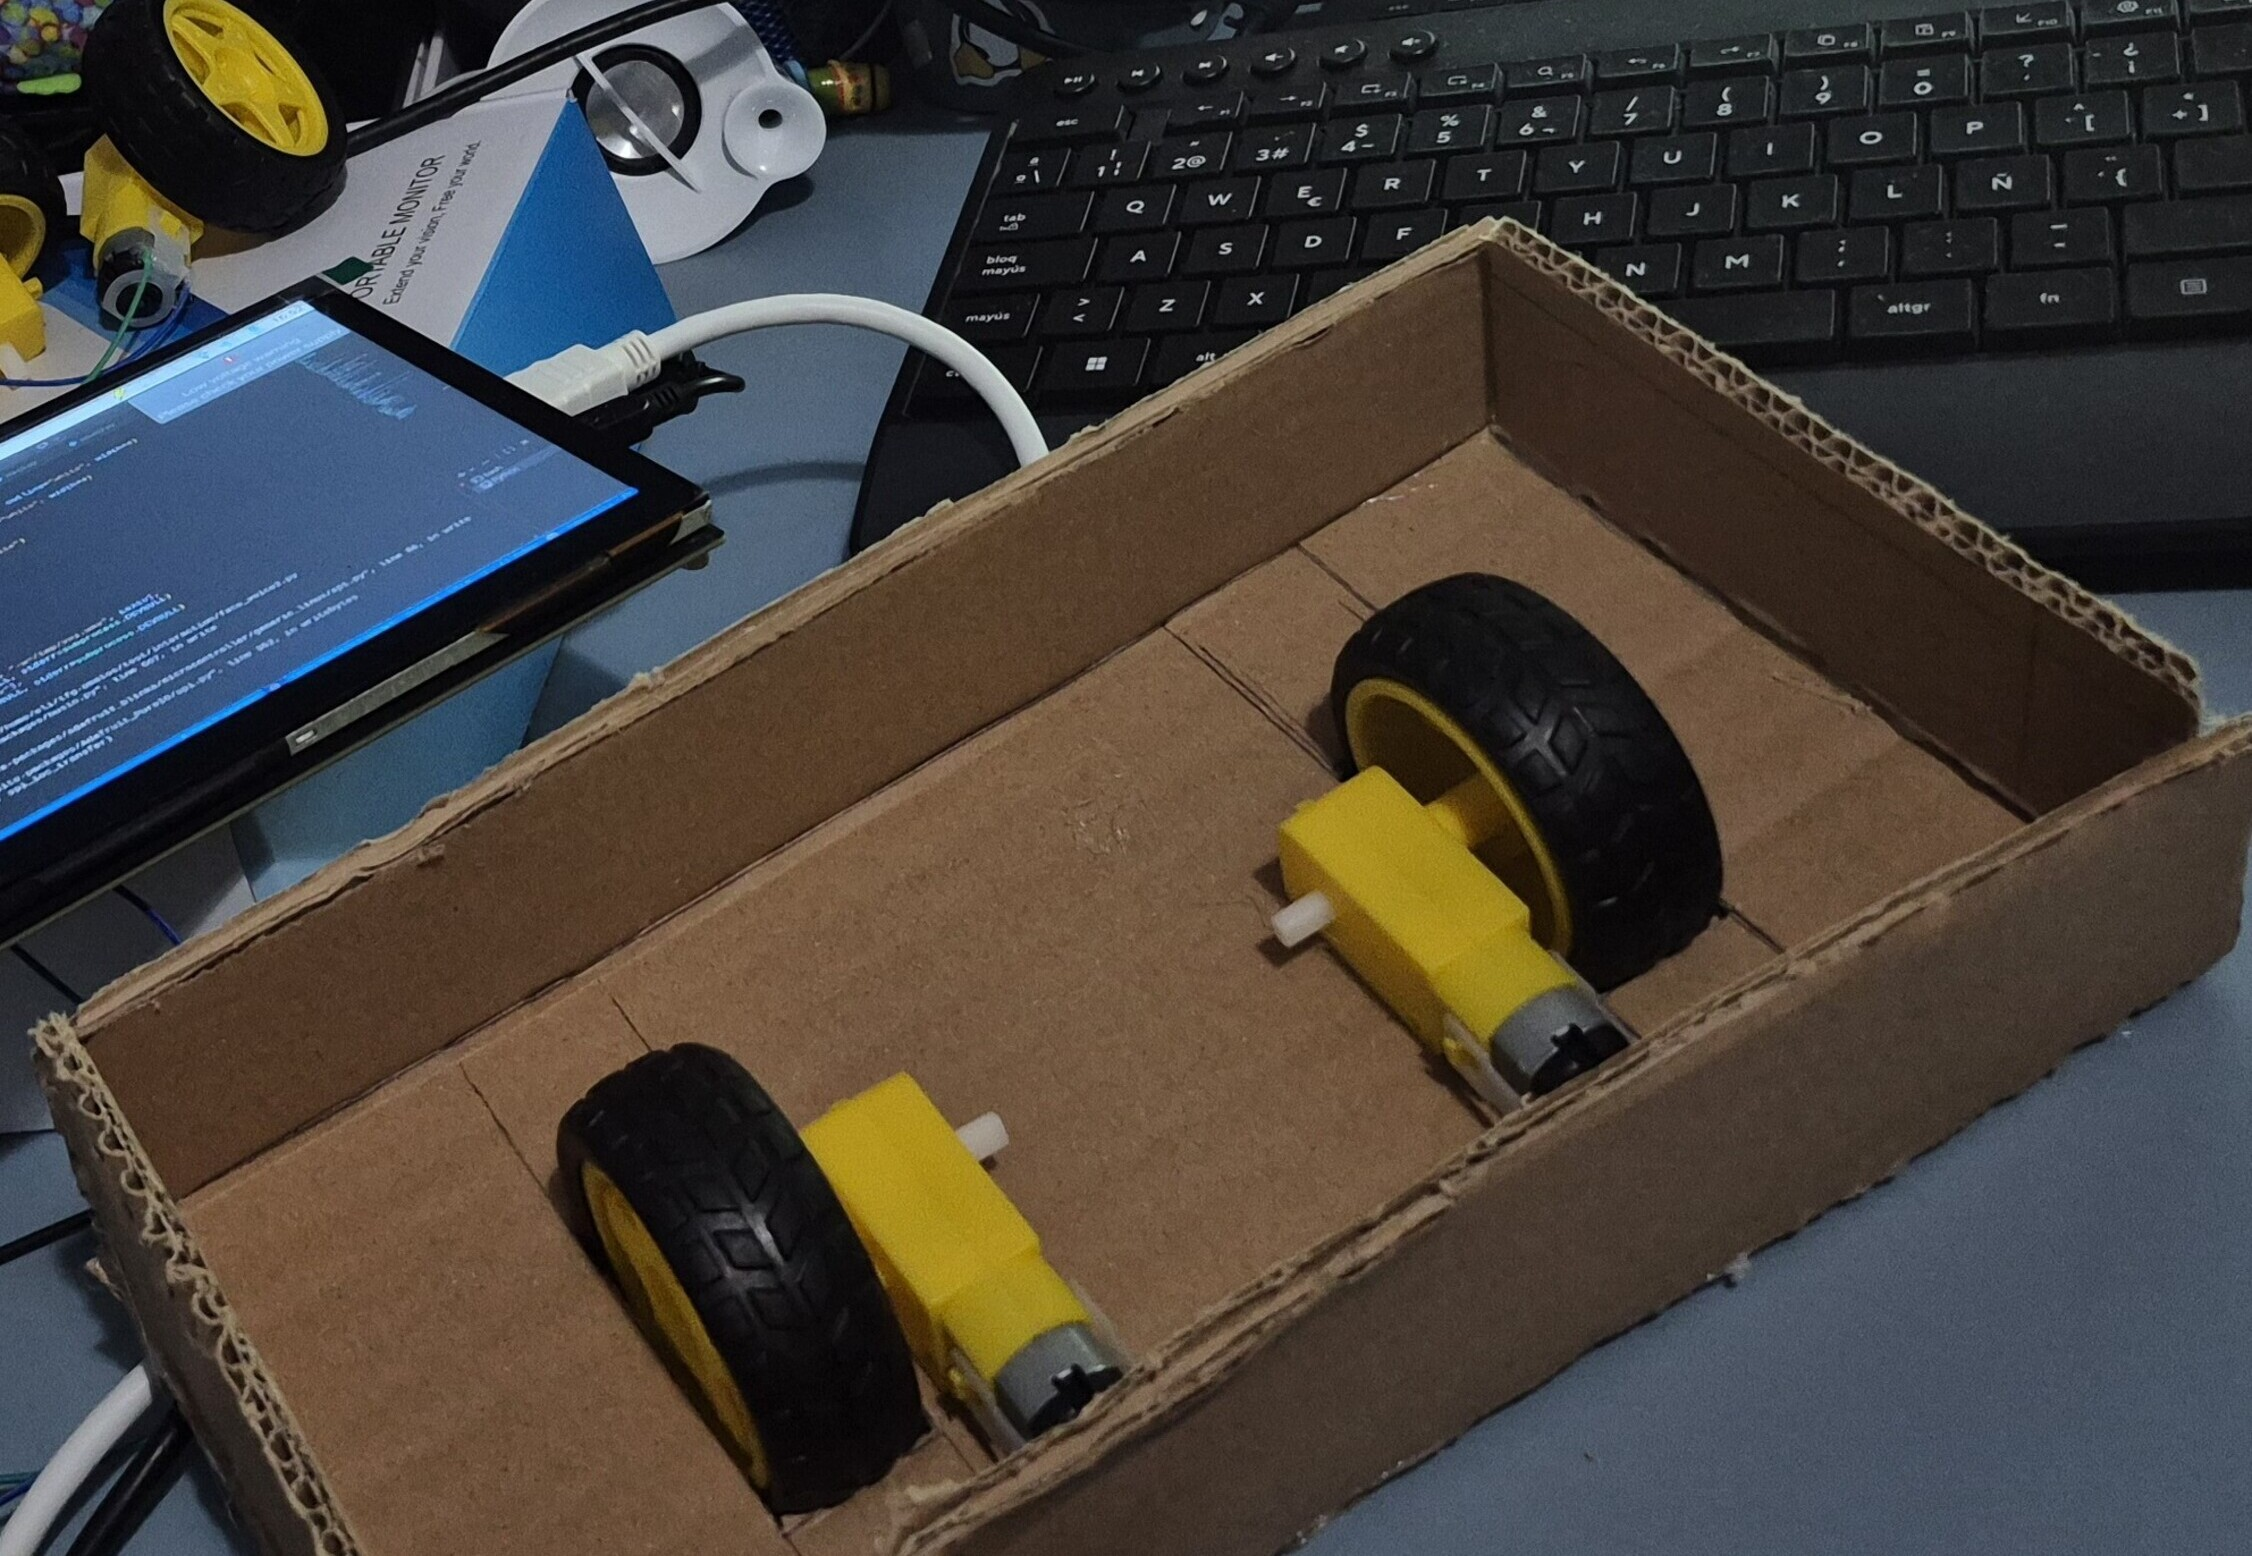
\includegraphics[height=3.6cm]{figs/ruedas_carton}

\end{figure}
\end{frame}


\begin{frame}
\frametitle{Modelo 3D}
\begin{figure}
\centering

\vspace{0.5cm}


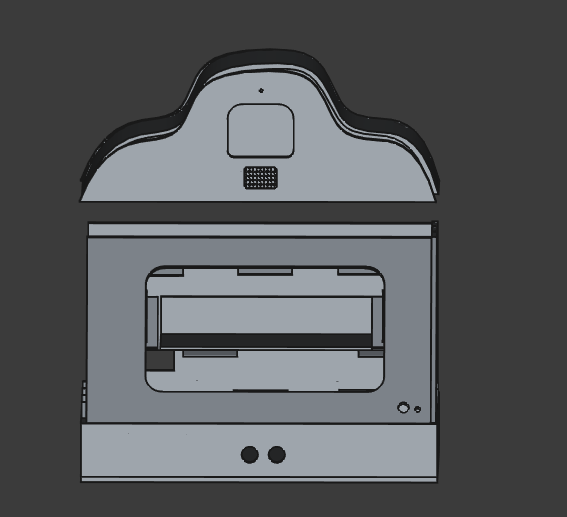
\includegraphics[height=3.6cm]{figs/3D2}
\hspace{0.4cm}
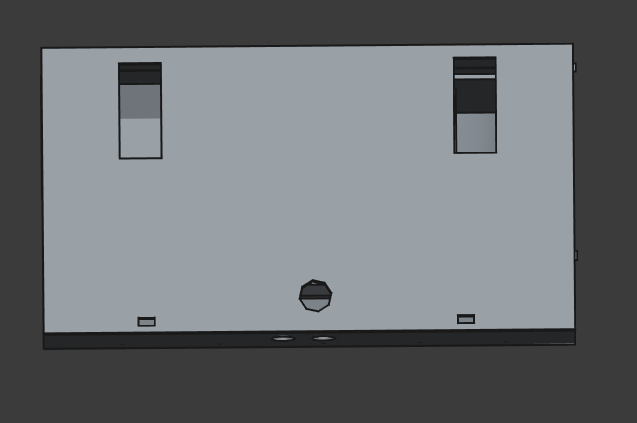
\includegraphics[height=3.6cm]{figs/3D3}

\end{figure}
\end{frame}



\begin{frame}
\frametitle{Estructura final del robot}
\begin{figure}
\centering

\vspace{0.5cm}

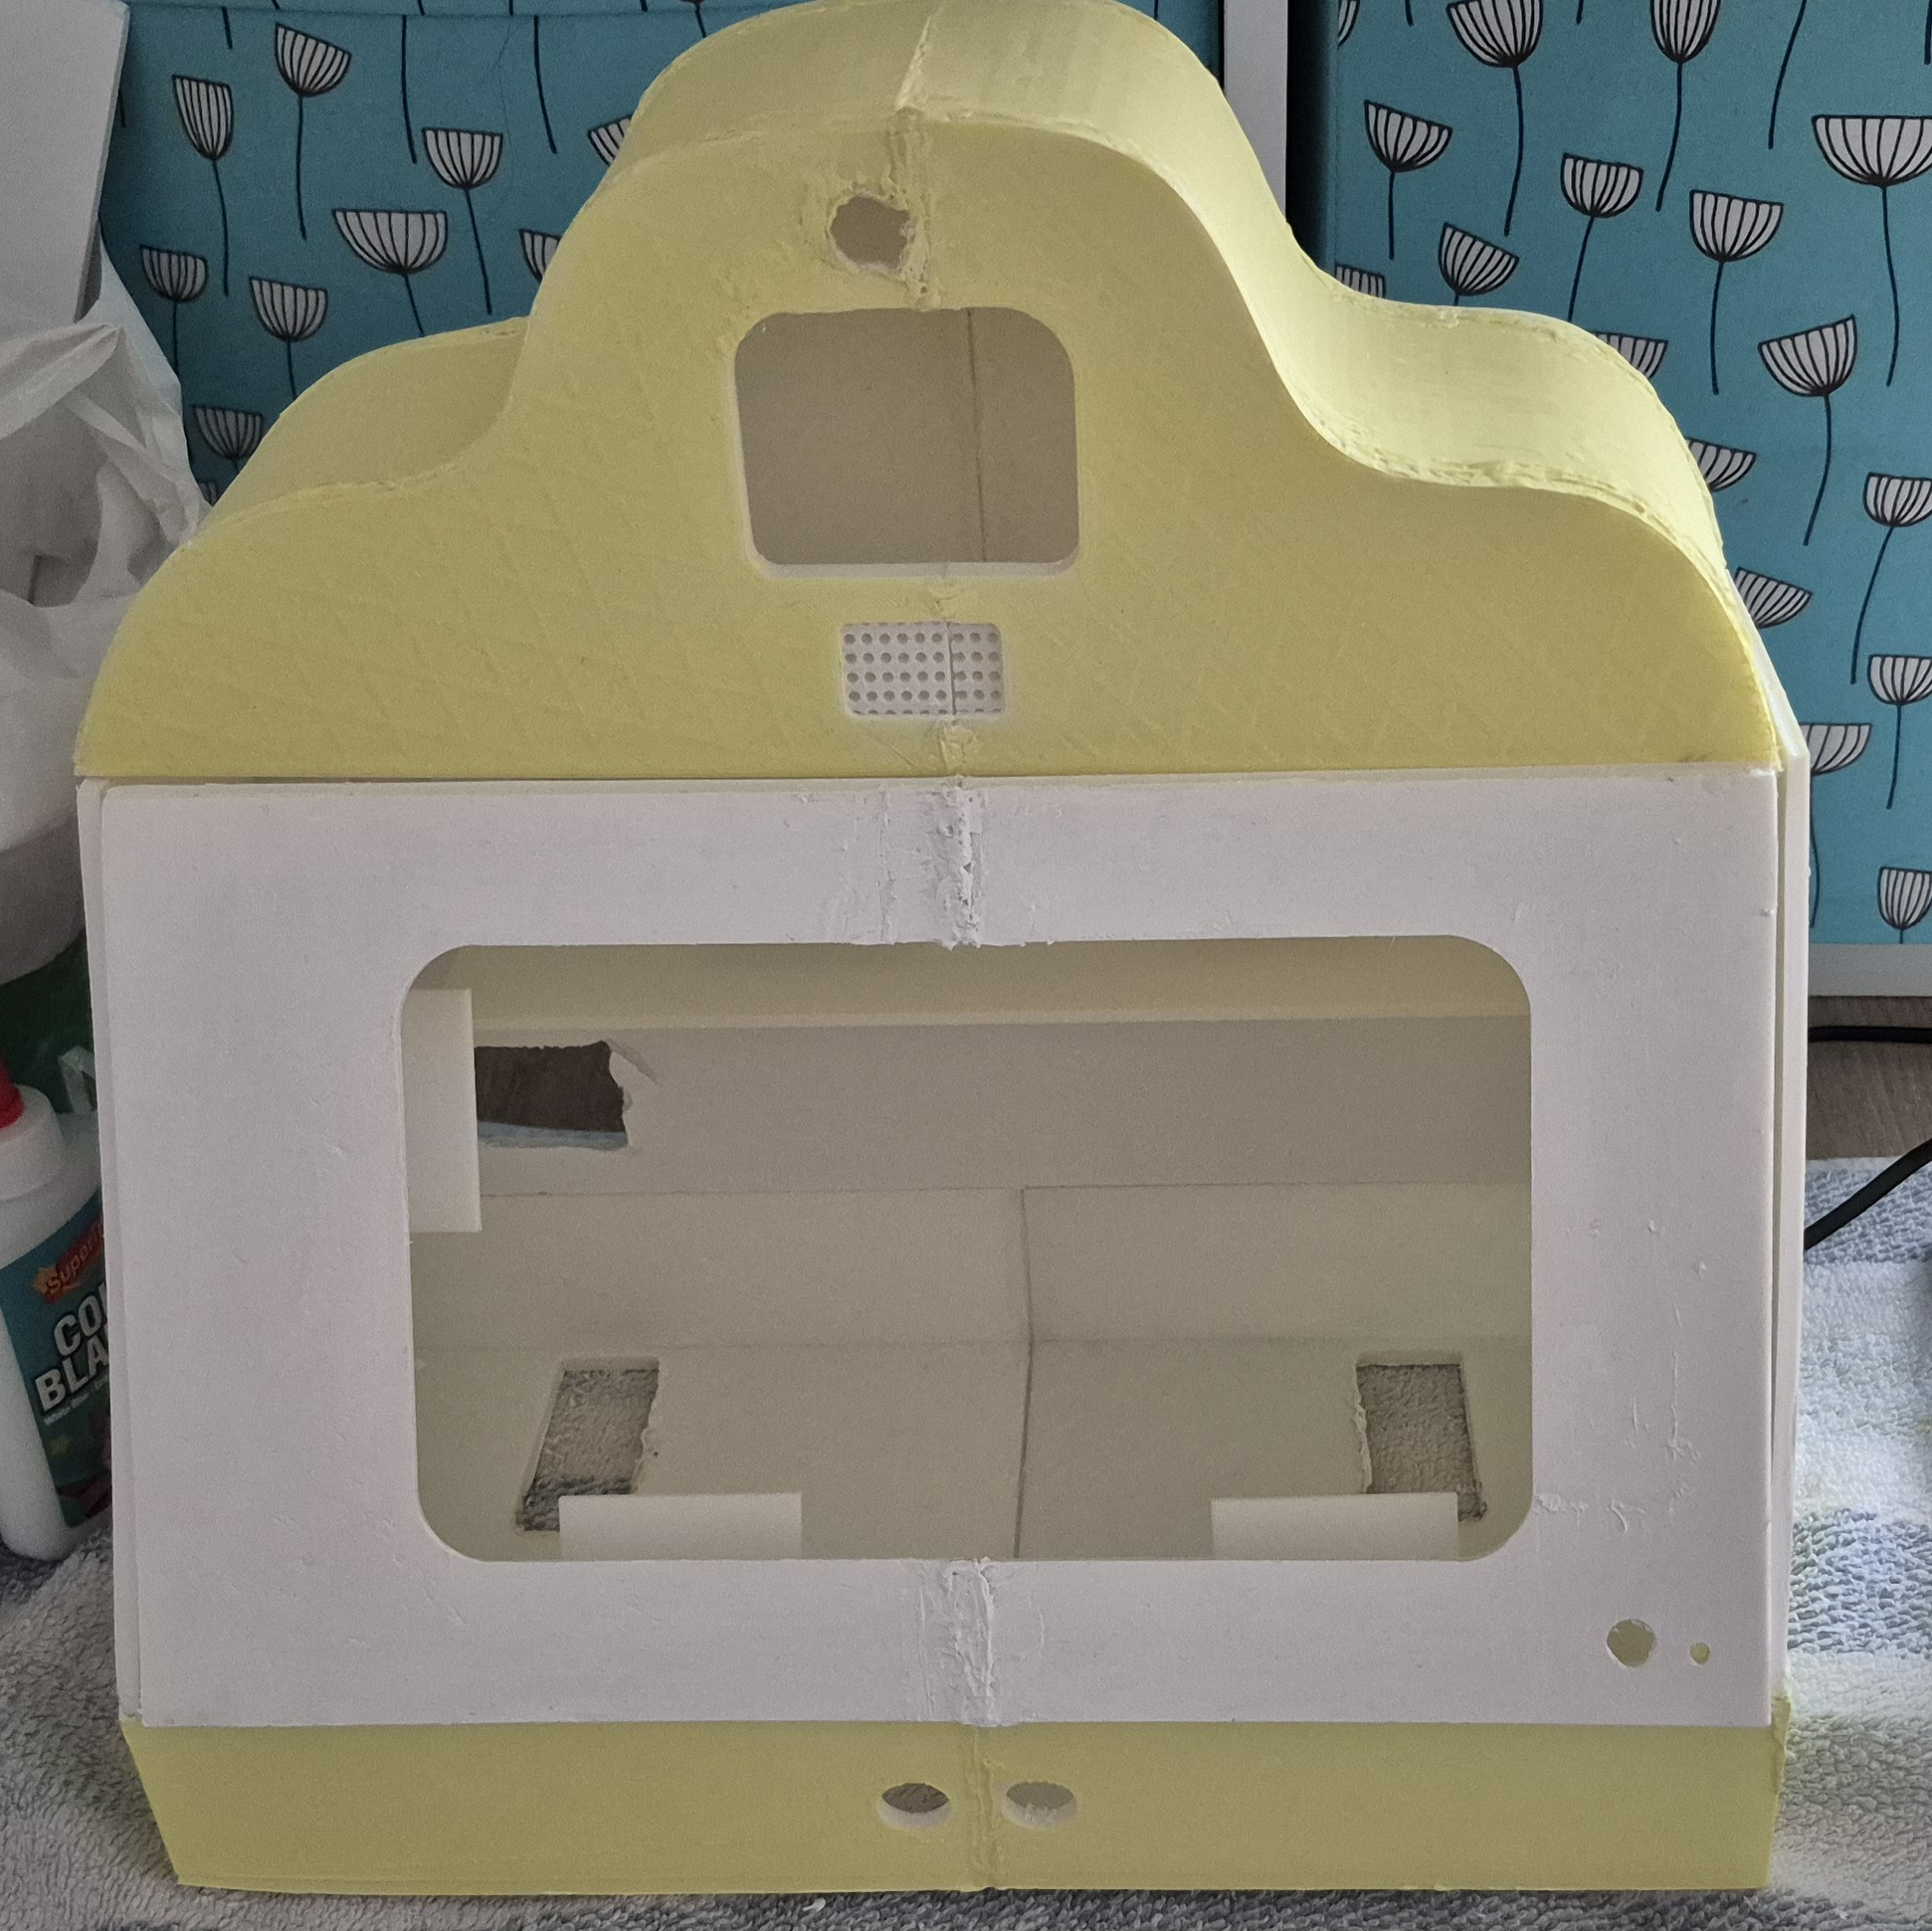
\includegraphics[height=5cm]{figs/estructura1}

\end{figure}
\end{frame}



\section*{}
\begin{frame}{}
  \centering \Huge
  \emph{Arquitectura software del sistema}
\note[item]{Pasemos ahora a comentar los objetivos que nos hemos con este trabajo.}
\end{frame}

\section{Arquitectura software del sistema}

\begin{frame}
\frametitle{Tipología software}
\begin{figure}
\centering
\begin{block}{Características}
\begin{itemize}

\note[item]{el código está dividido en diferentes modulos}
\note[item]{cada módulo se encarga de una funcialidad diferente}
\note[item]{facilitando el mantenimiento del código}


\item \alert{Modularización} del código.

\end{itemize}
\end{block}

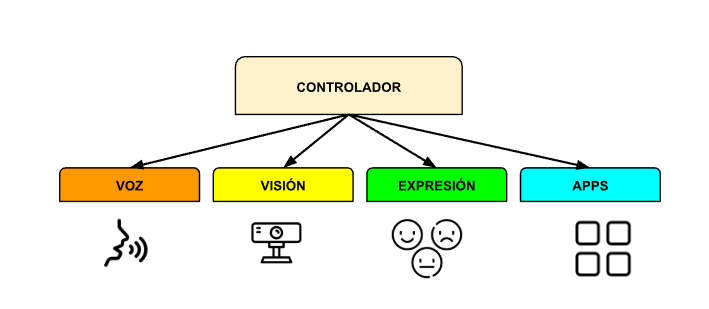
\includegraphics[height=5cm]{figs/mod}

\end{figure}
\end{frame}



\begin{frame}
\frametitle{Tipología software}
\begin{figure}
\centering
\begin{block}{Características}
\begin{itemize}

\item Diseño \alert{distribuido}.

\end{itemize}
\end{block}

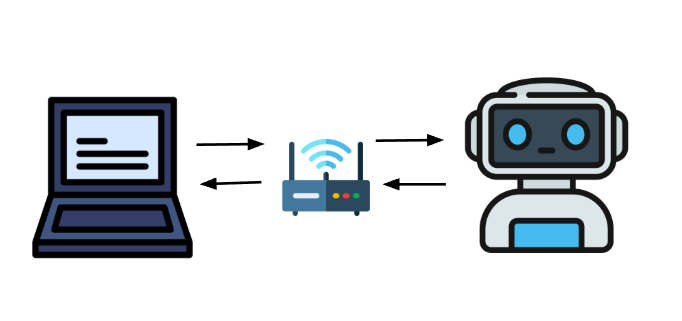
\includegraphics[height=4.8cm]{figs/wifi}

\end{figure}
\end{frame}


\begin{frame}
\frametitle{Servidor}
\begin{figure}
\centering

\vspace{0.1cm}


\includegraphics[height=5.8cm]{figs/server}

\end{figure}
\end{frame}



\begin{frame}
\frametitle{Interfaz de usuario}
\begin{figure}
\centering


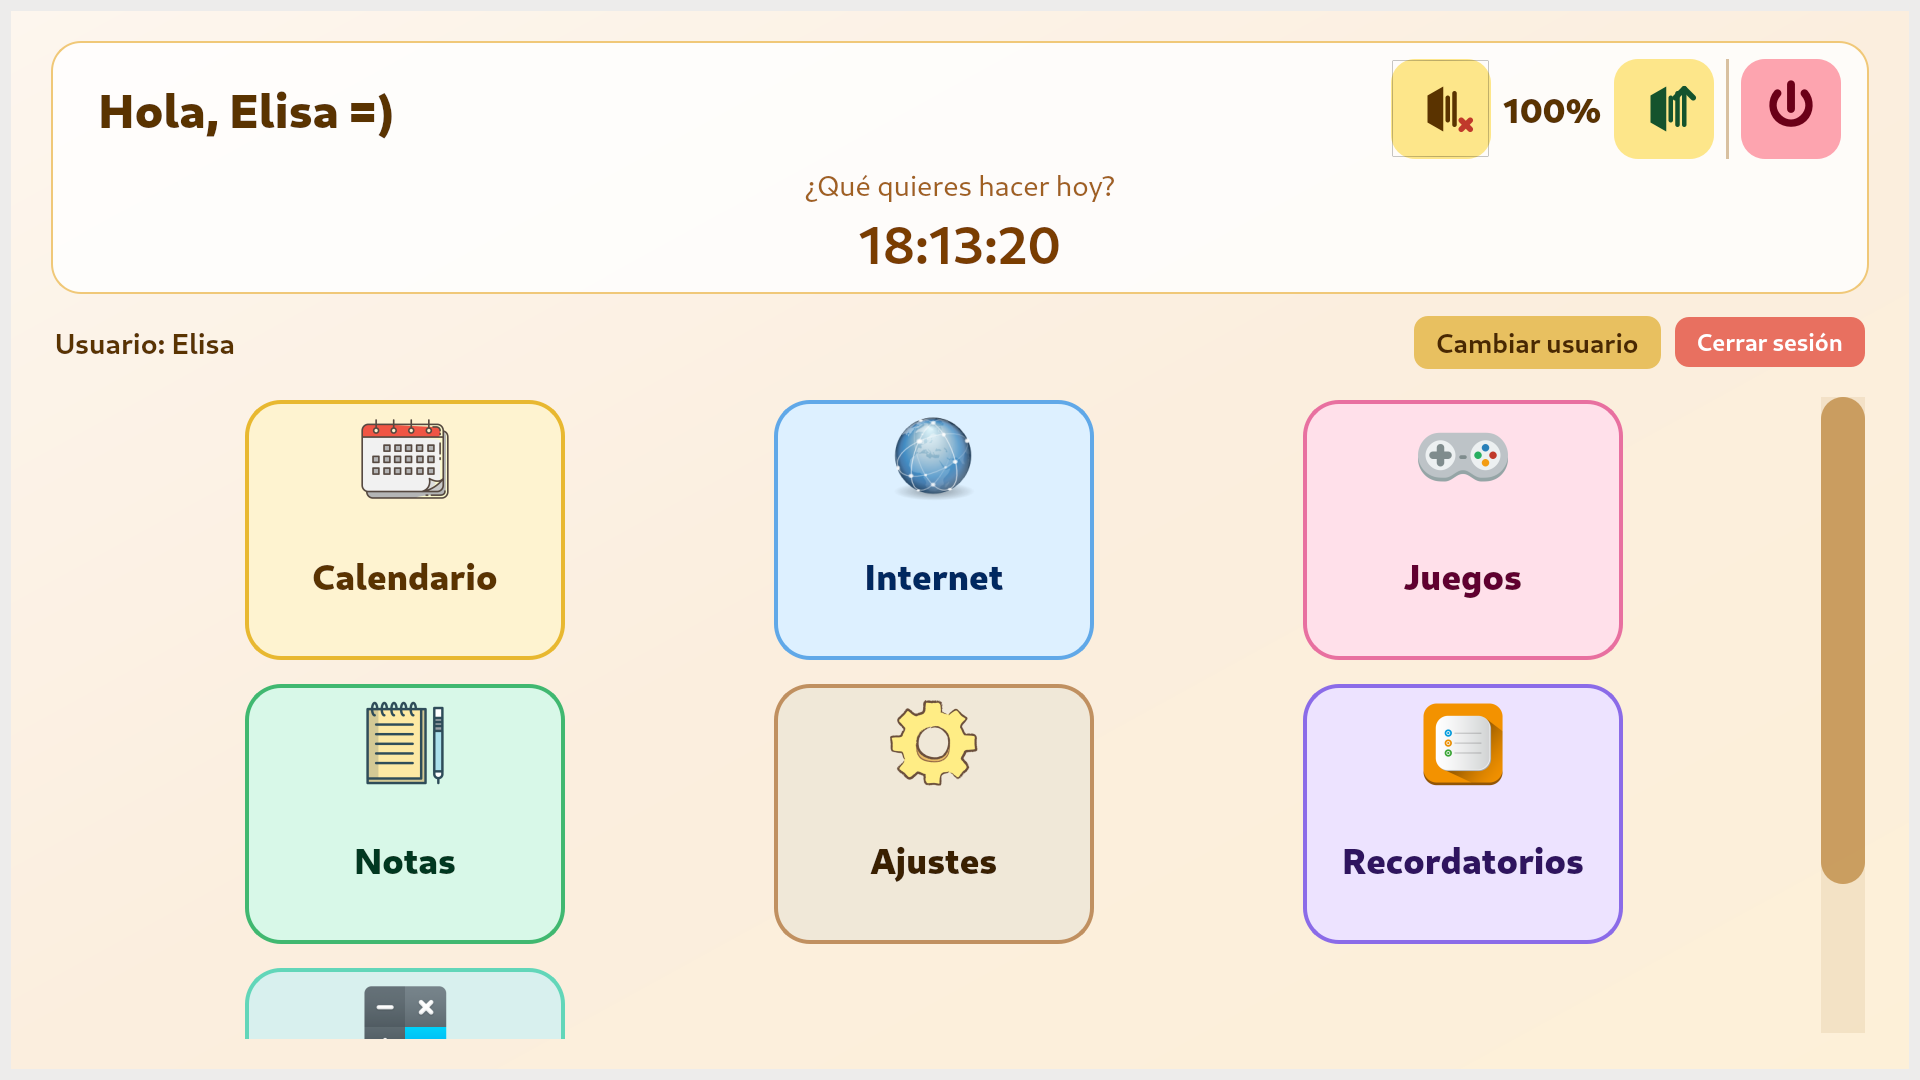
\includegraphics[width=0.45\textwidth]{figs/launch}
\hspace{0.02\textwidth}
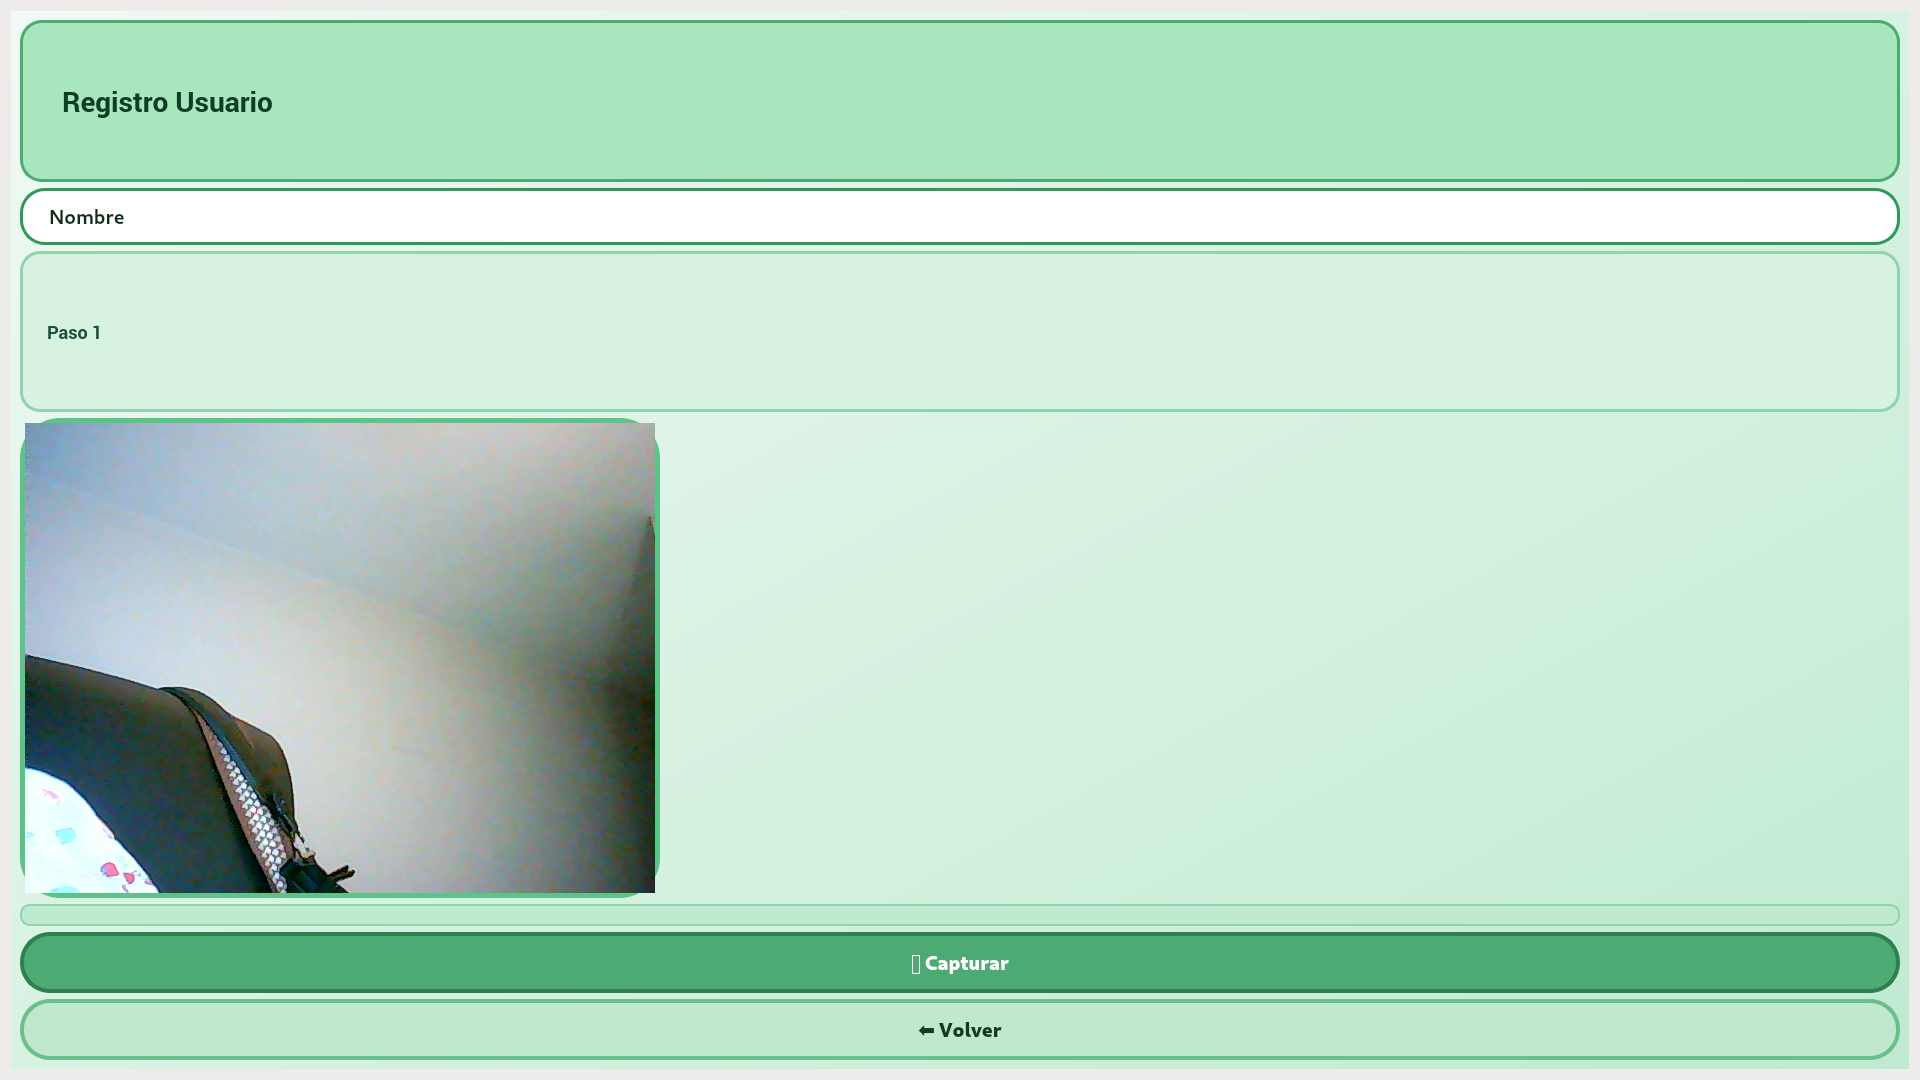
\includegraphics[width=0.45\textwidth]{figs/cap}

\end{figure}
\end{frame}

\begin{frame}
\frametitle{Interacción con el robot}
\begin{figure}
\centering

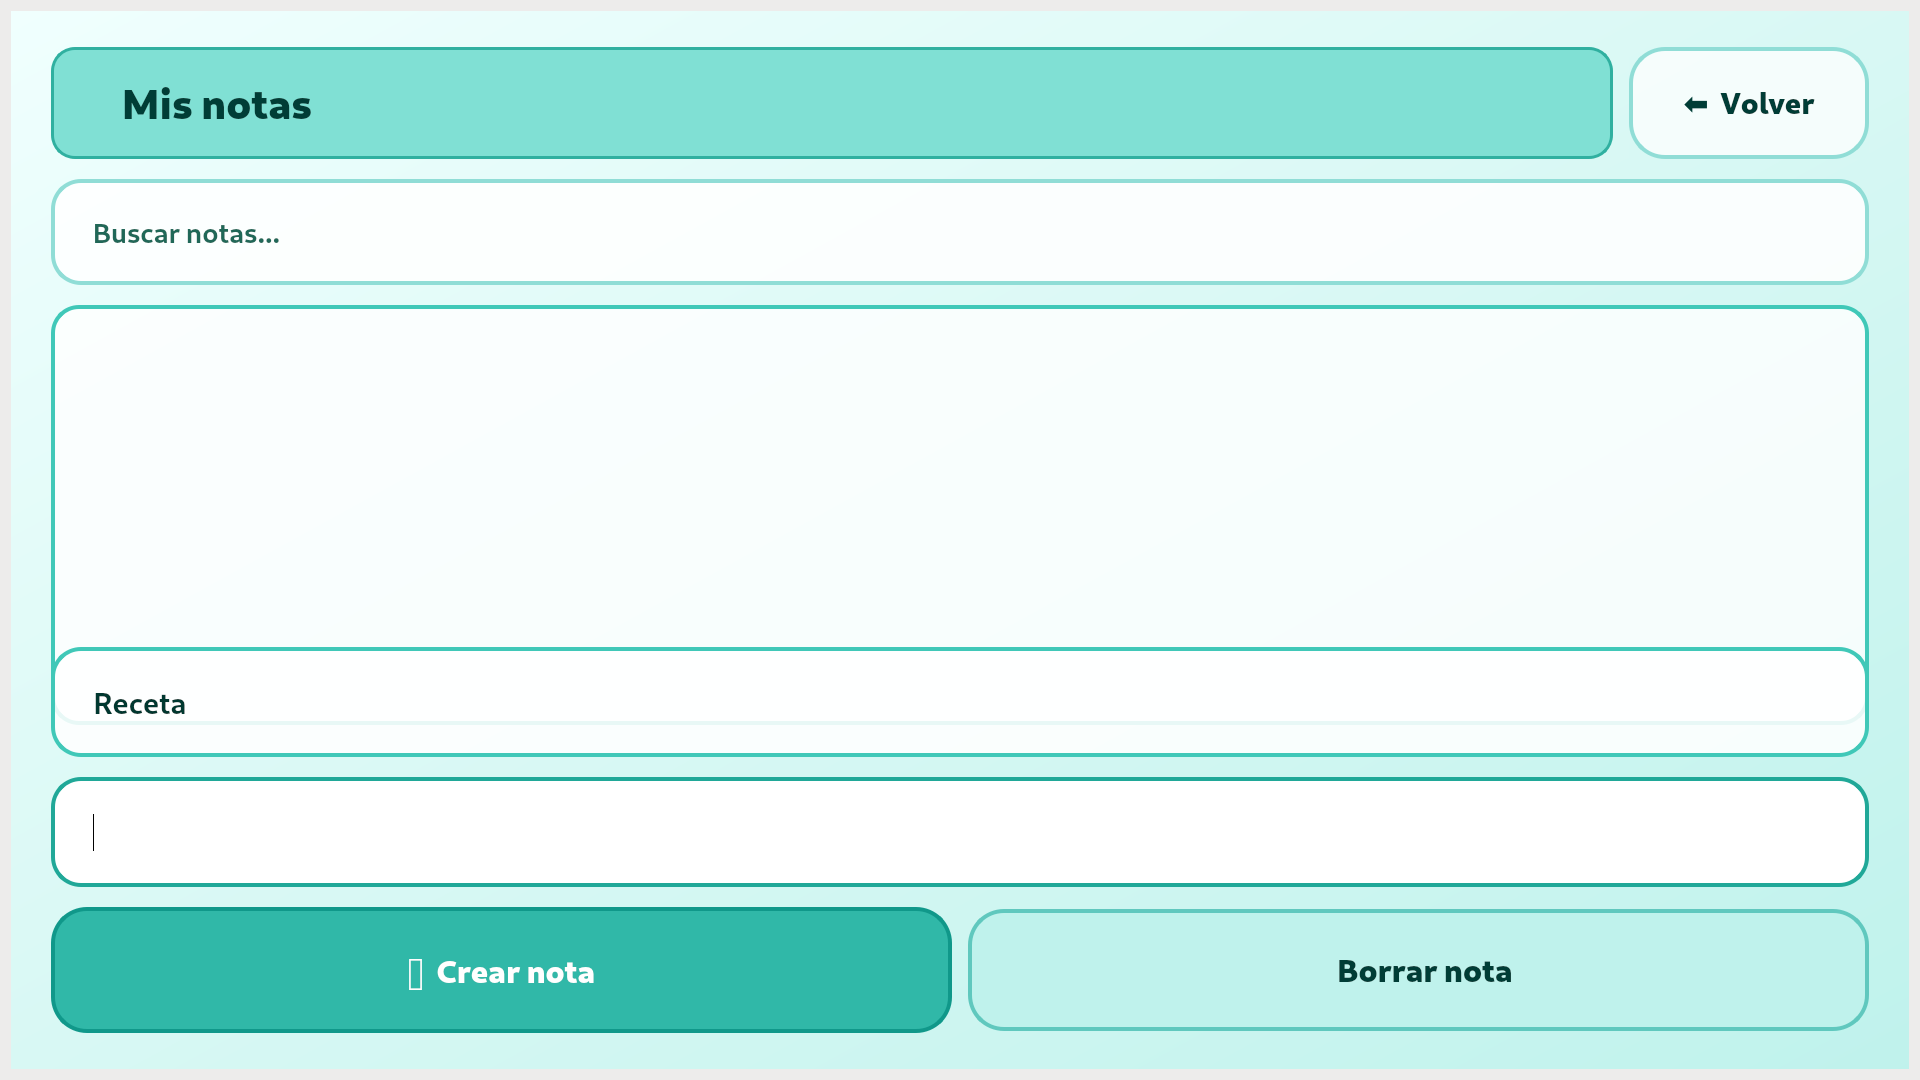
\includegraphics[width=0.45\textwidth]{figs/notas}
\hspace{0.02\textwidth}

\includegraphics[width=0.45\textwidth]{figs/cal}

\end{figure}
\end{frame}


\begin{frame}
\frametitle{Interfaz de usuario}
\begin{figure}
\centering

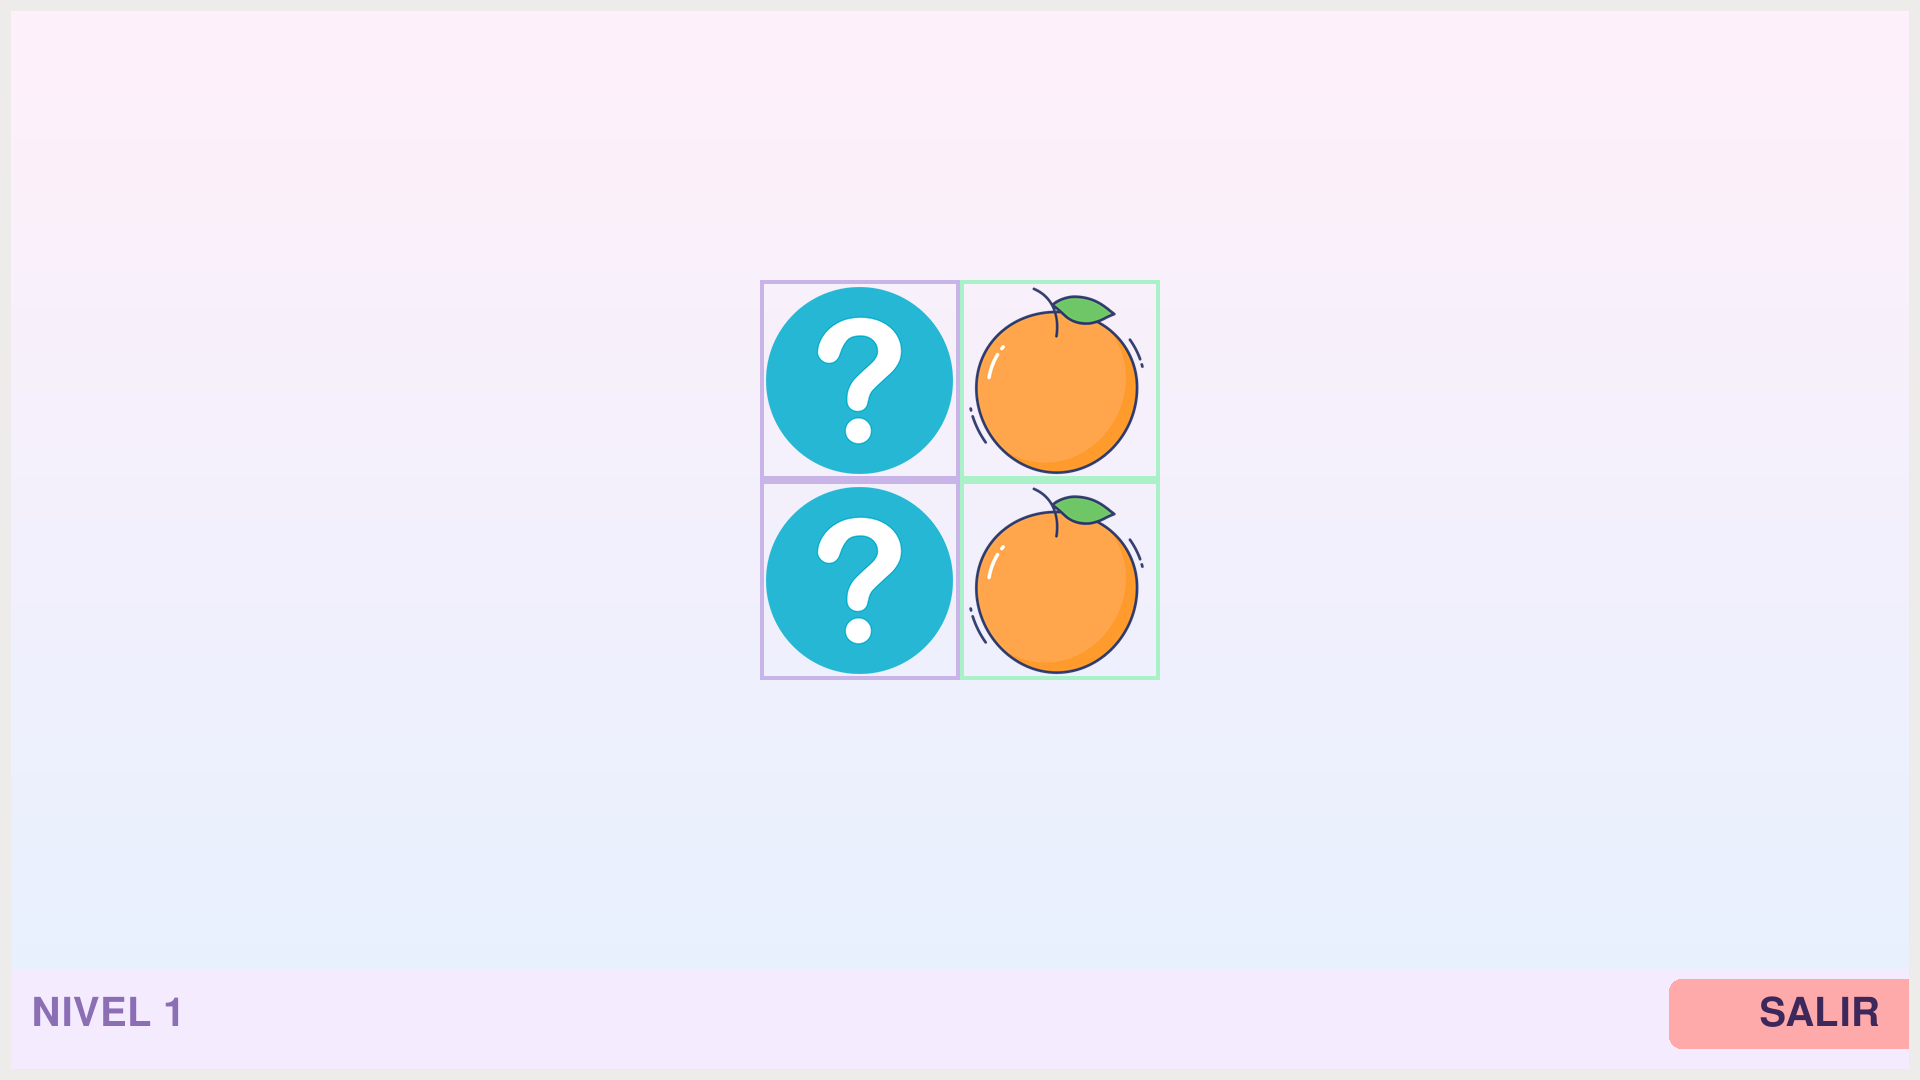
\includegraphics[width=0.45\textwidth]{figs/mem}
\hspace{0.02\textwidth}
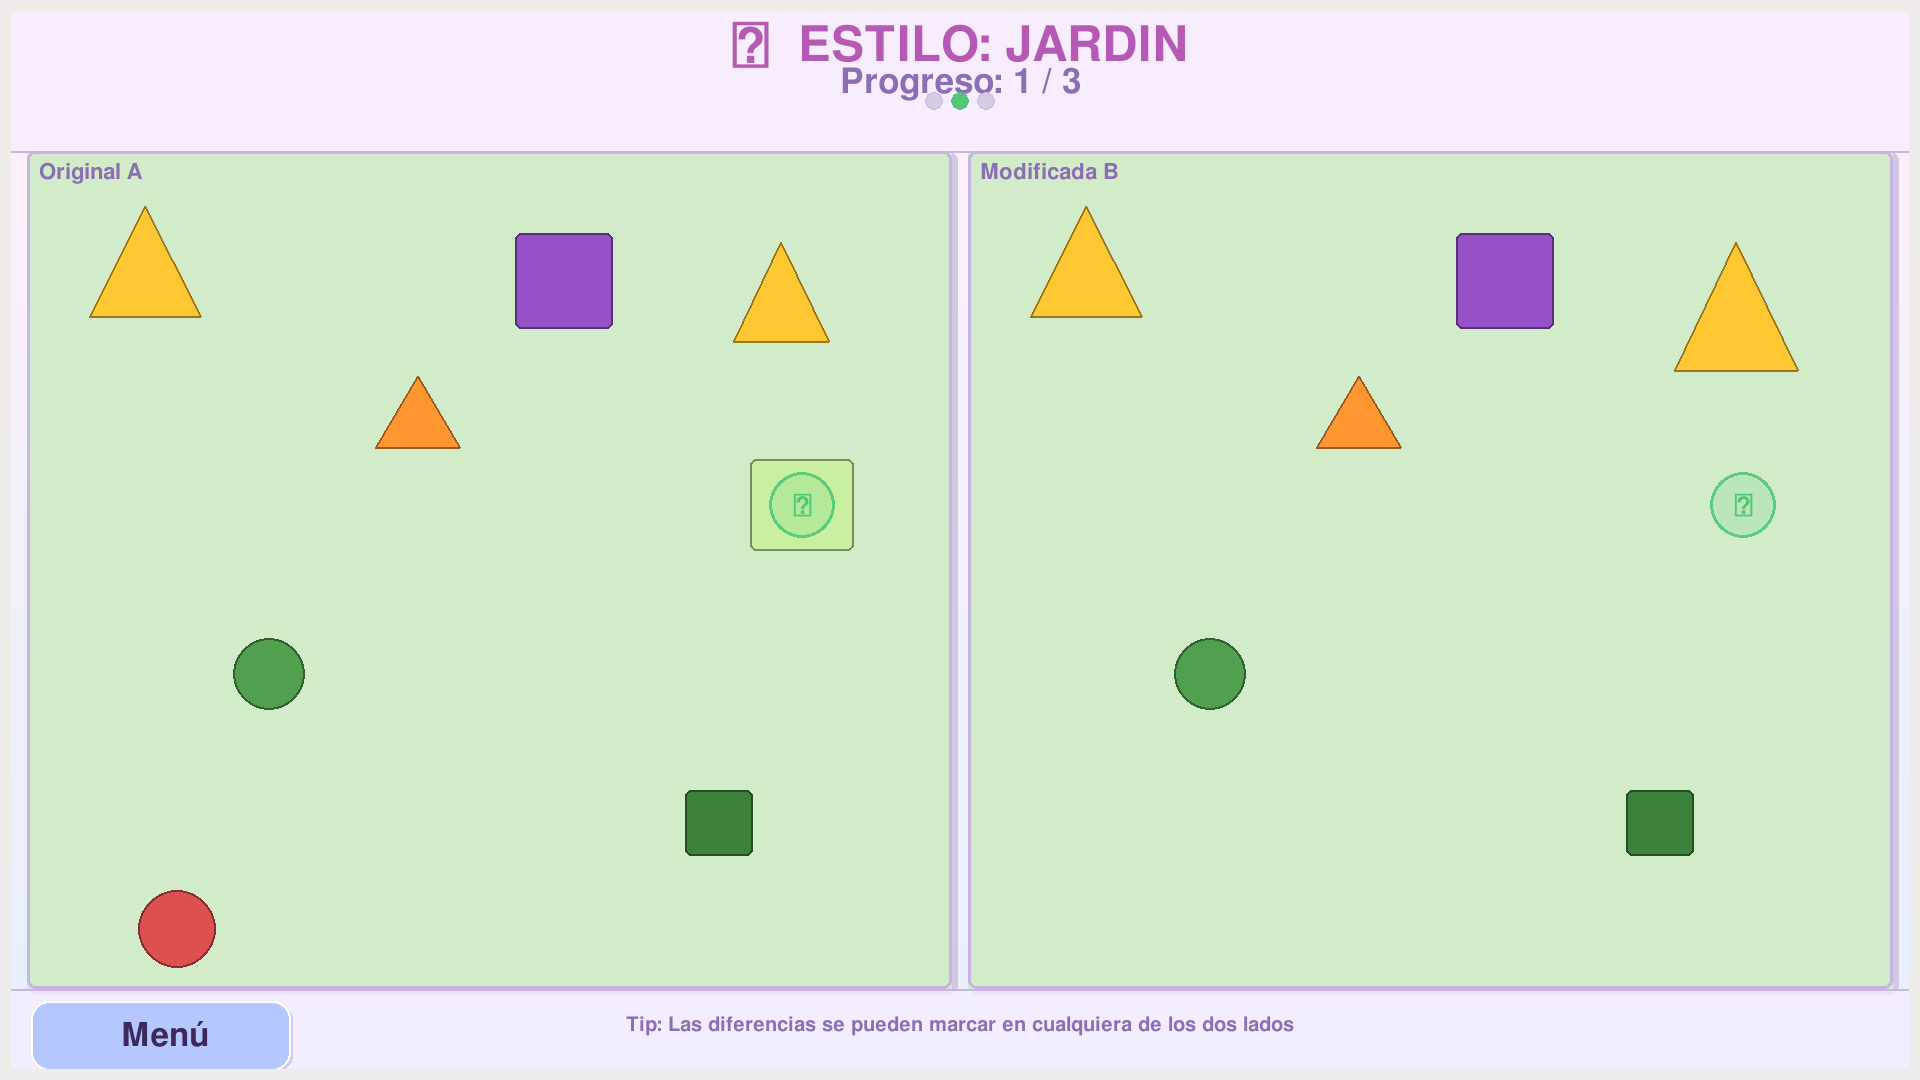
\includegraphics[width=0.45\textwidth]{figs/dif}

\end{figure}
\end{frame}

\begin{frame}
\frametitle{Interfaz de usuario}
\begin{figure}
\centering

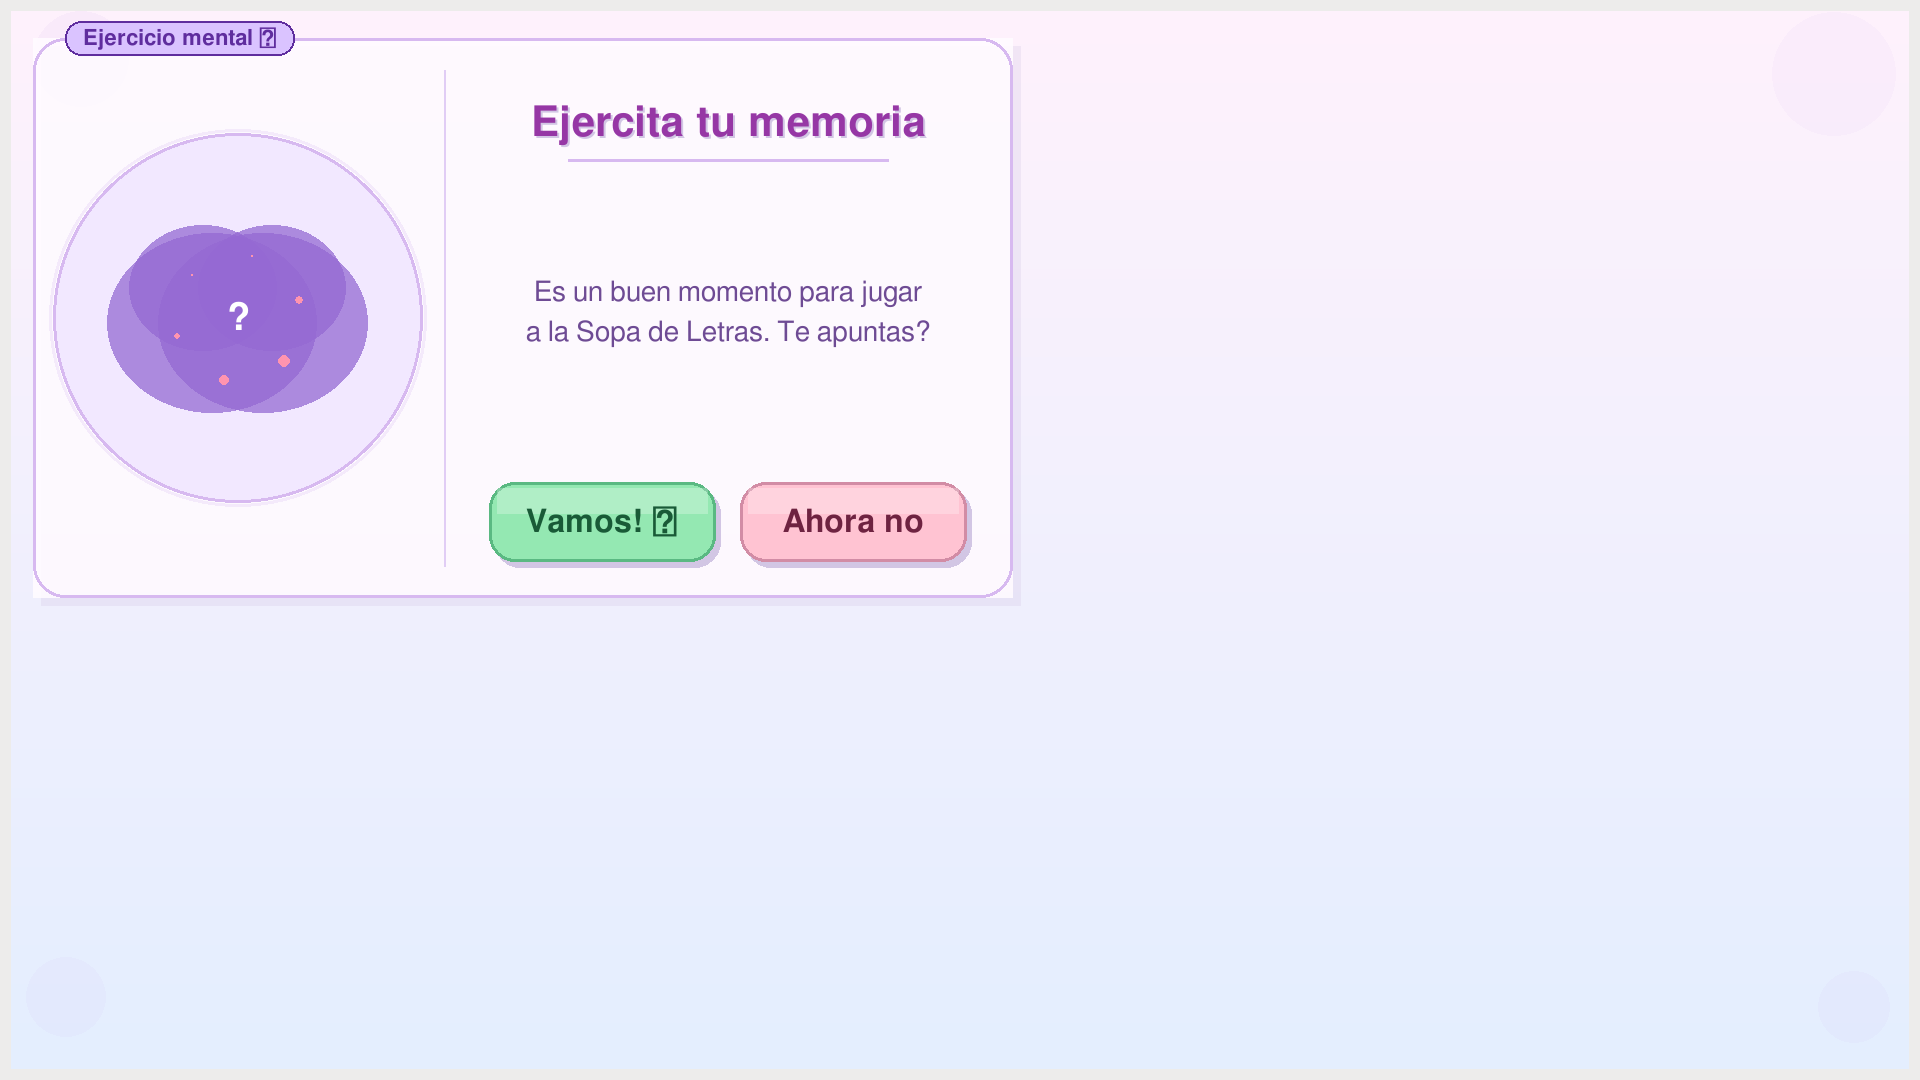
\includegraphics[width=1\textwidth]{figs/sugerencia}

\end{figure}
\end{frame}

\begin{frame}
\frametitle{Interacción con el robot}
\begin{figure}
\centering

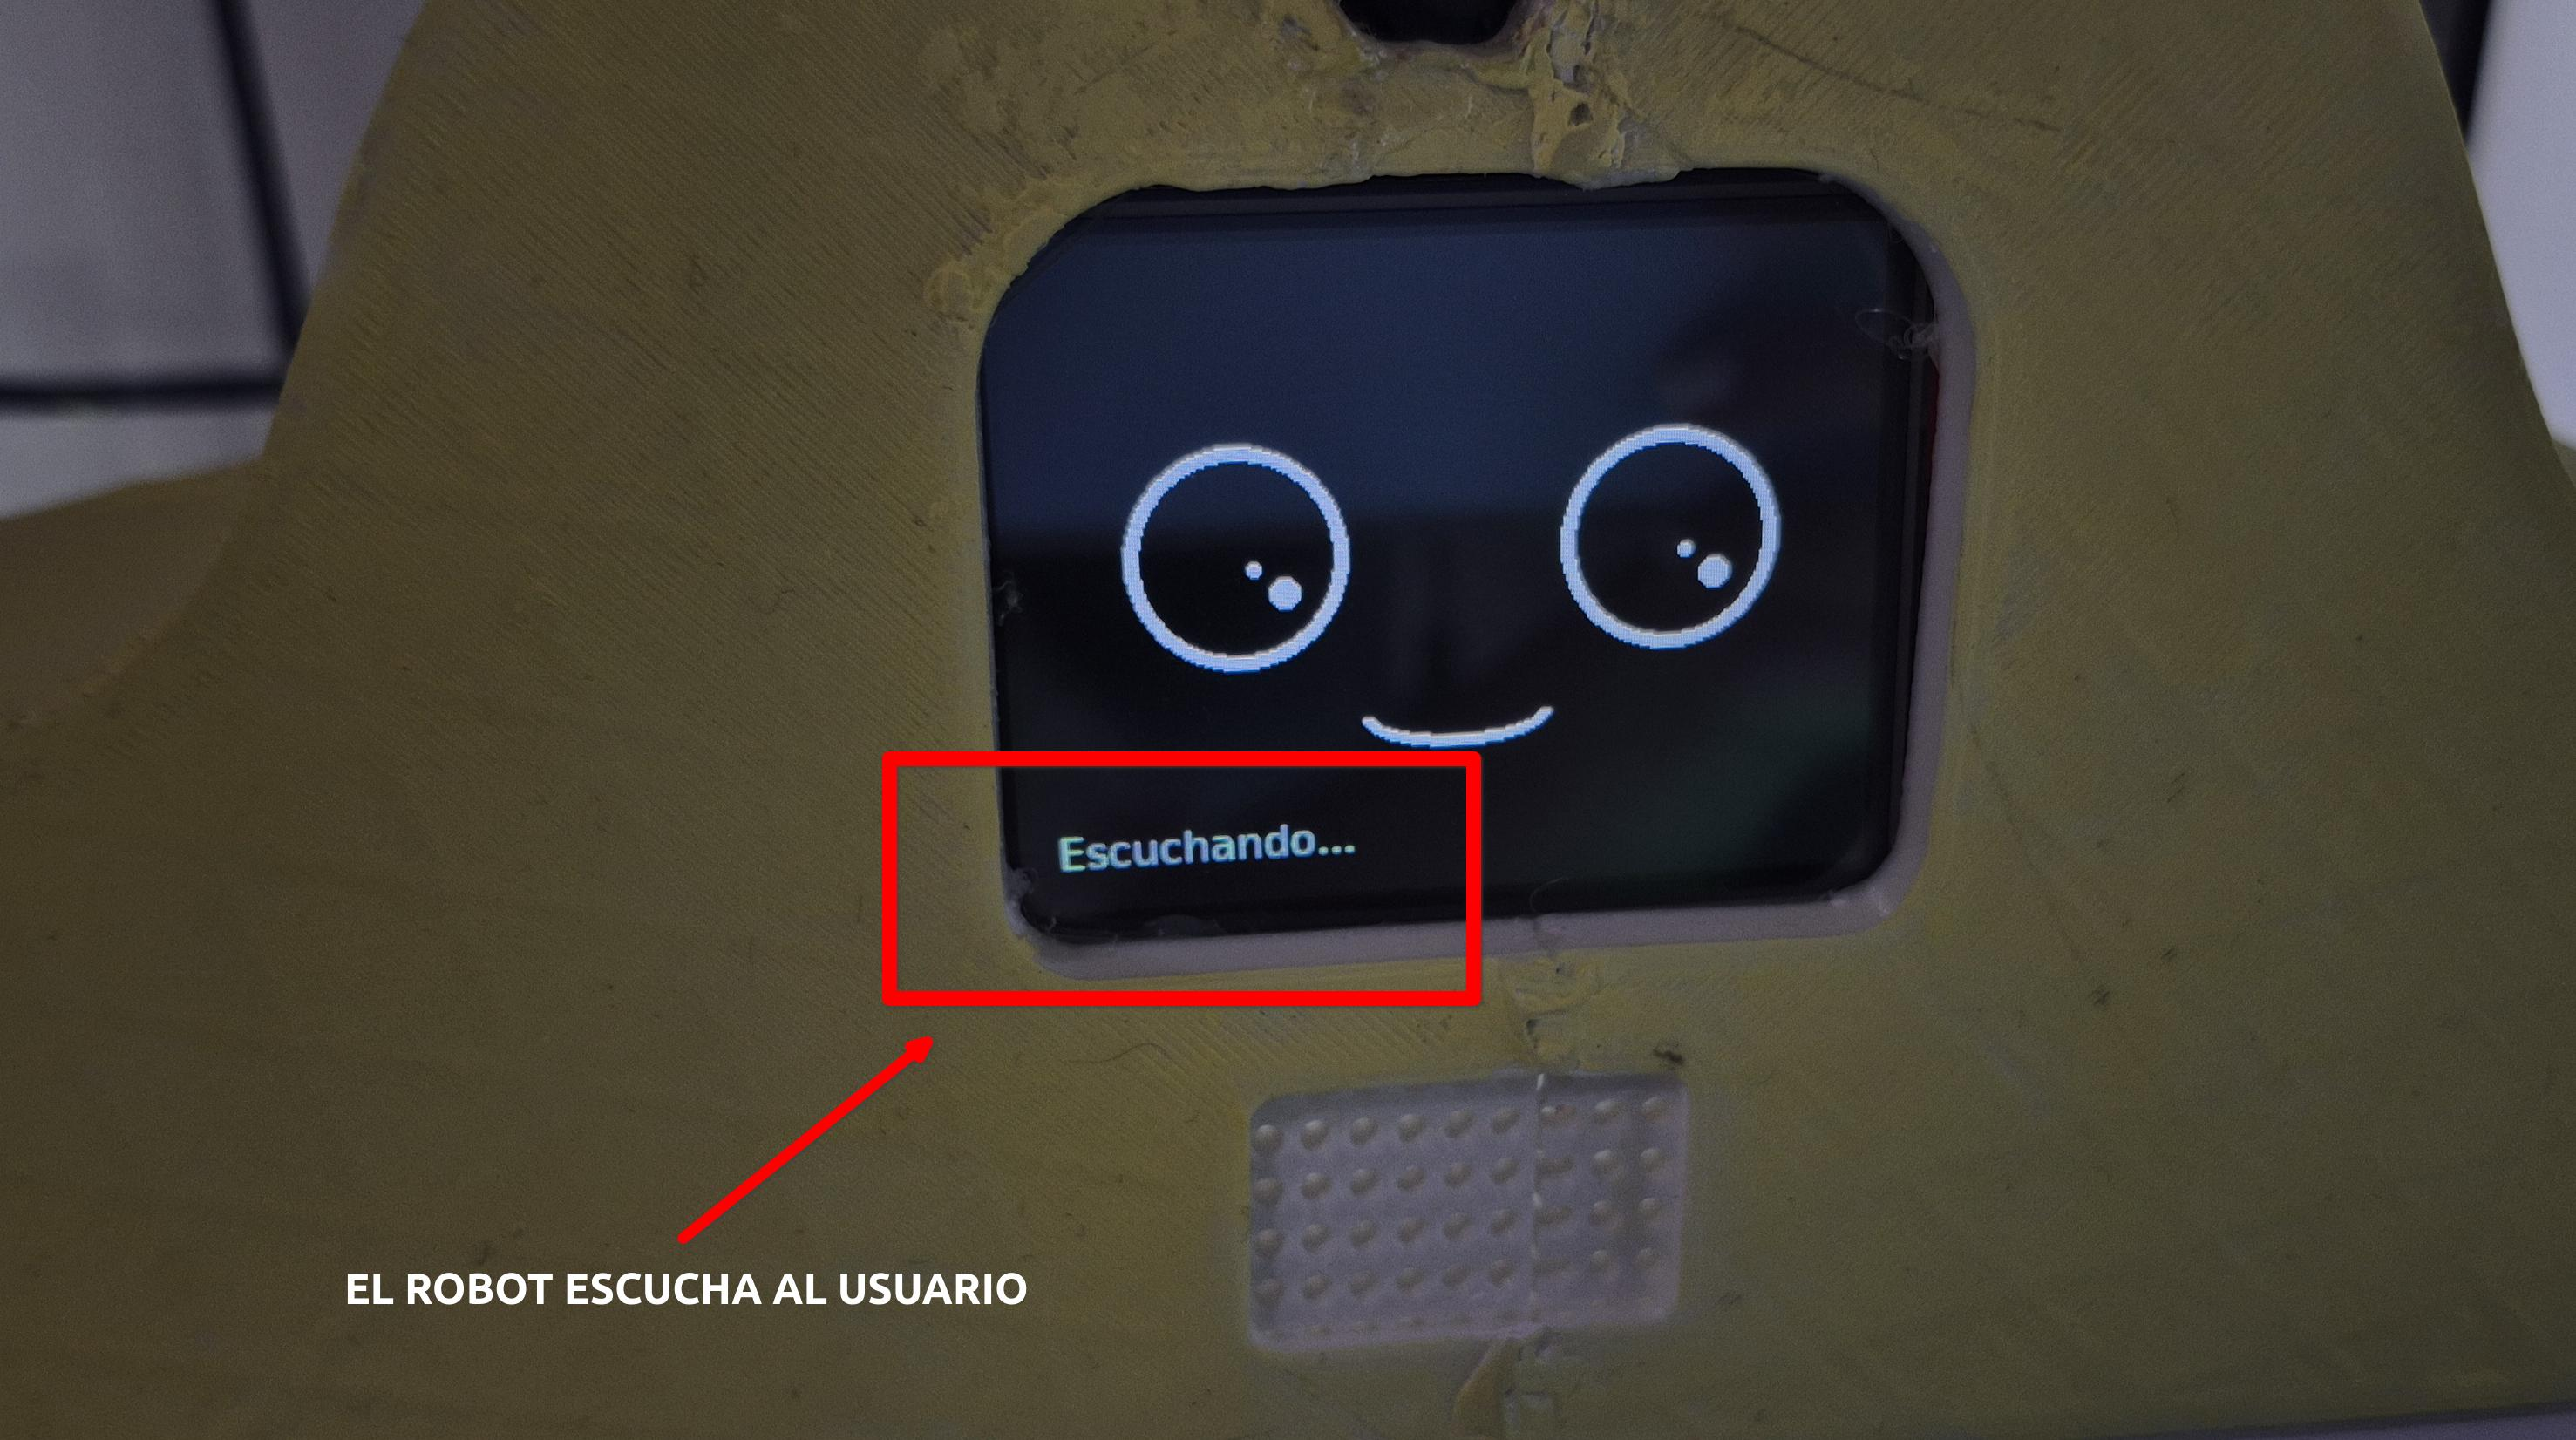
\includegraphics[width=0.45\textwidth]{figs/esc}
\hspace{0.02\textwidth}
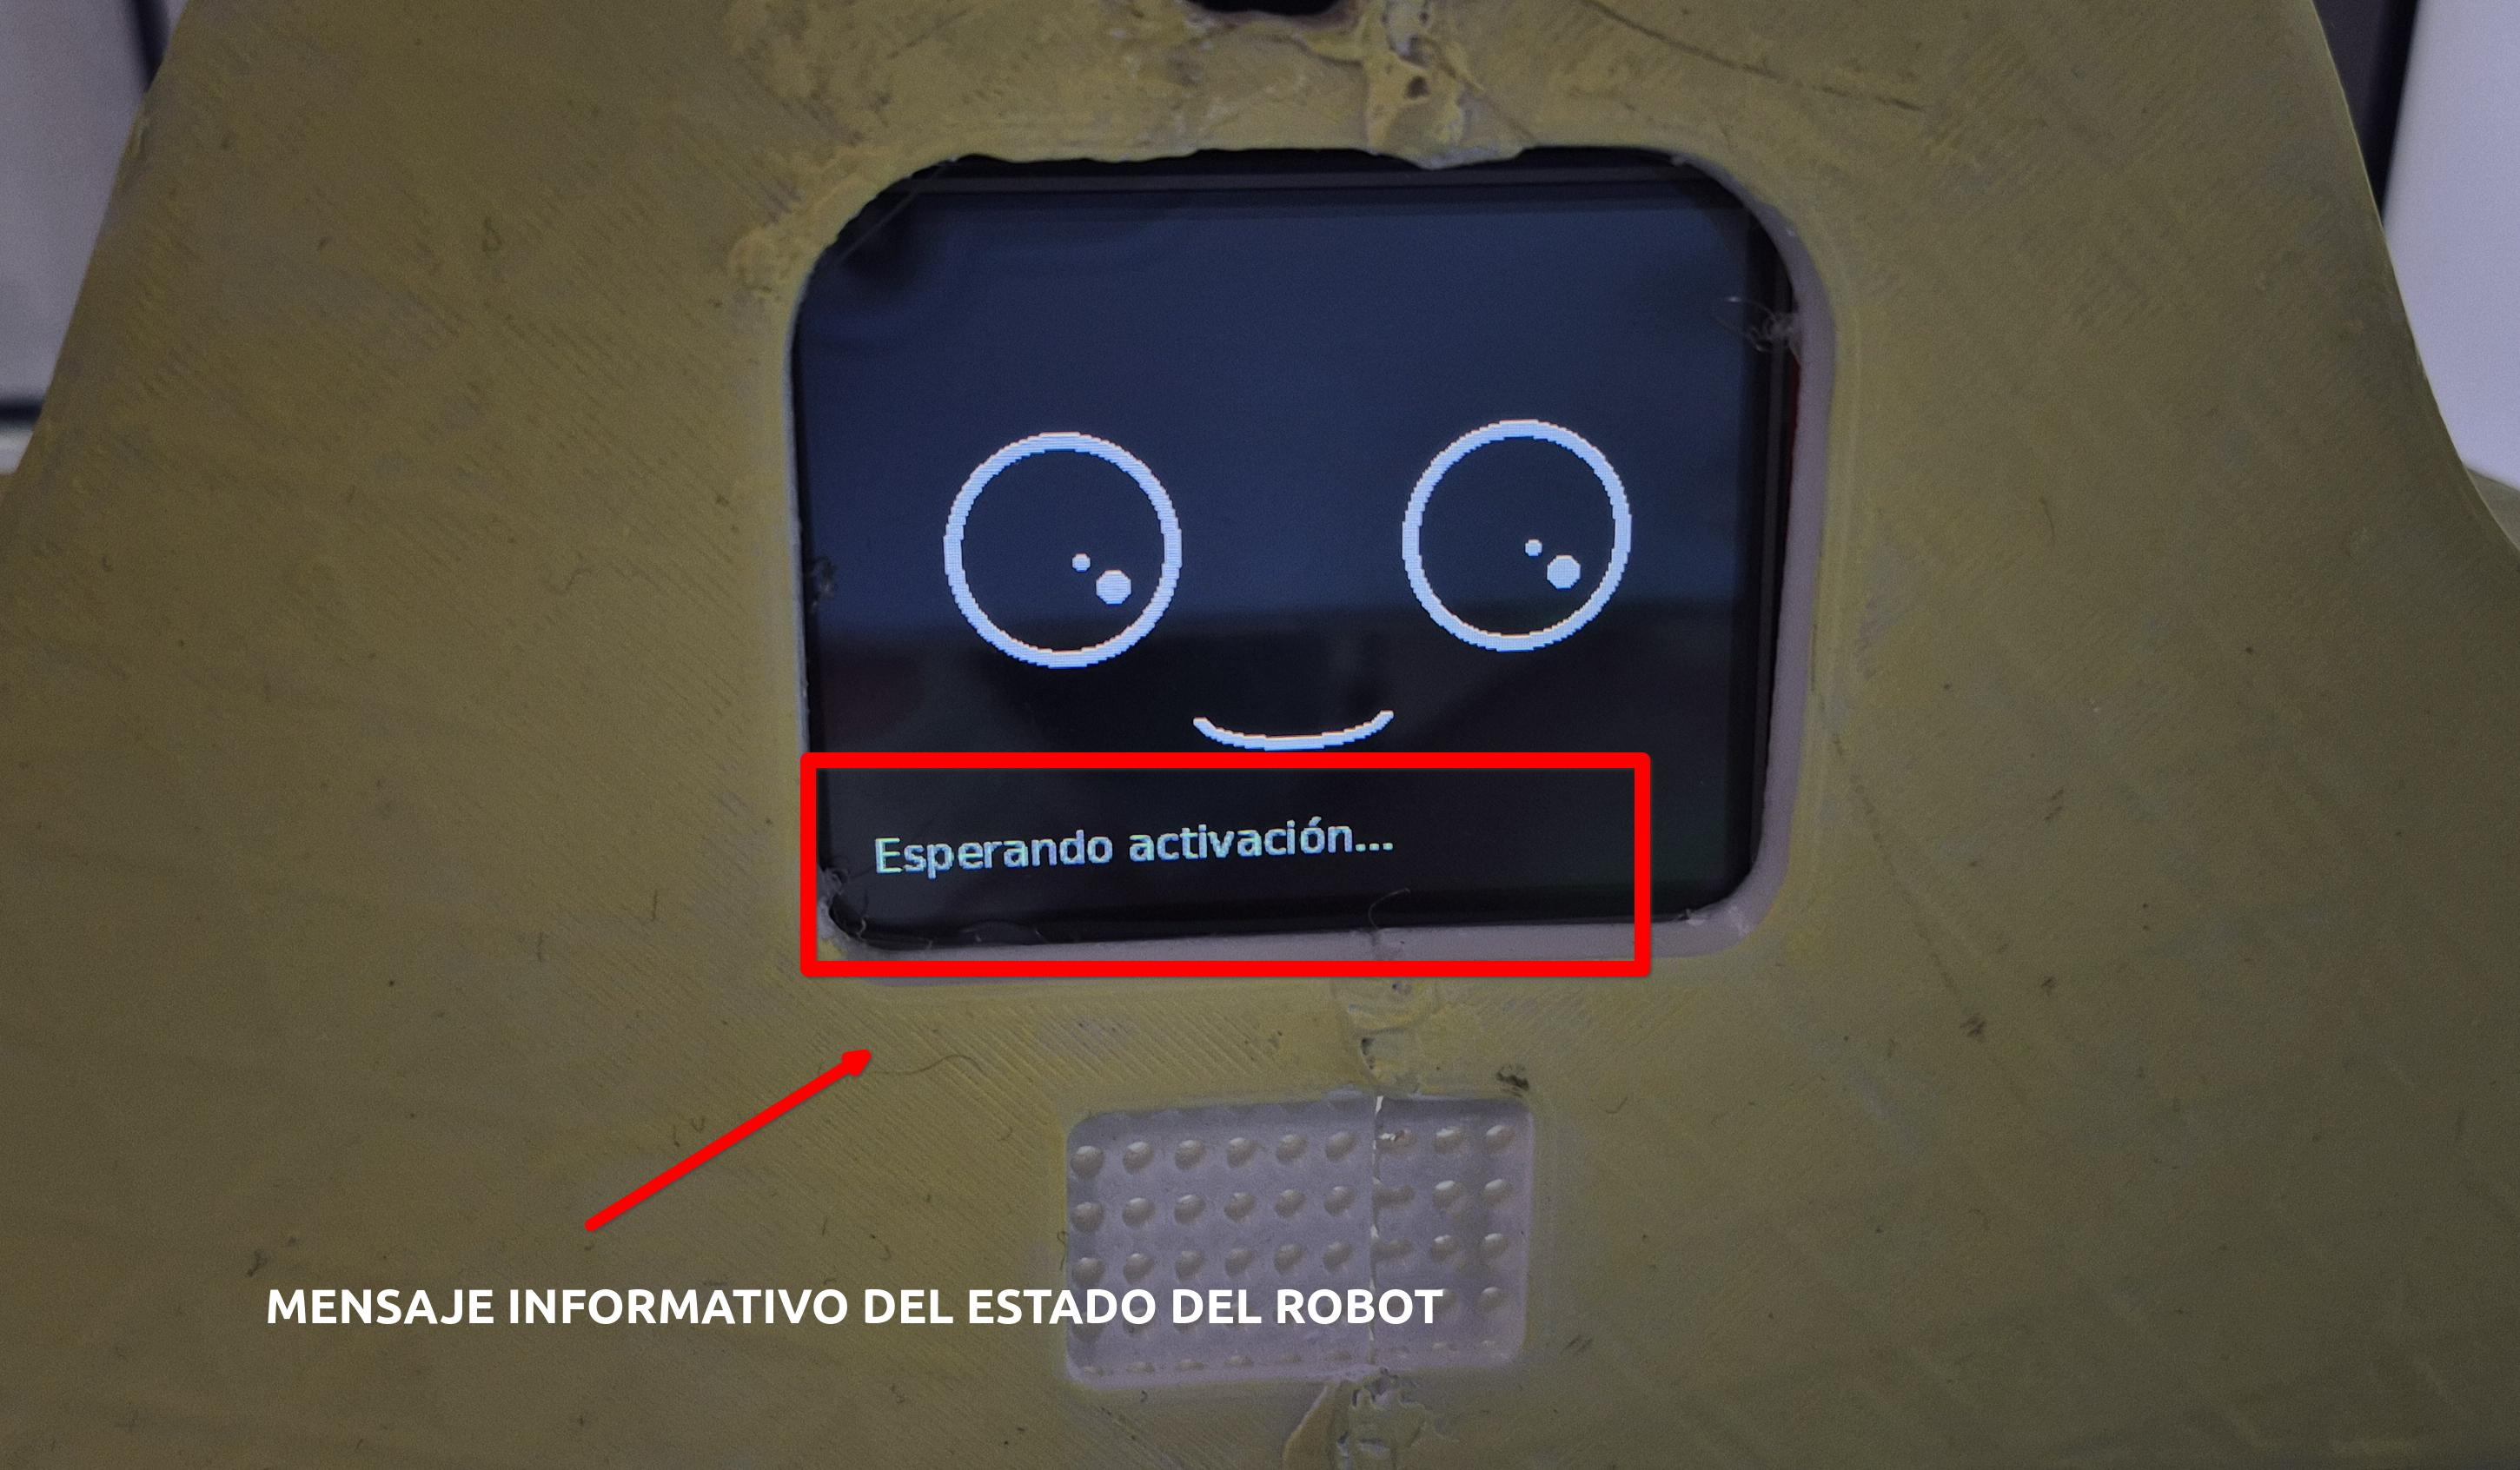
\includegraphics[width=0.45\textwidth]{figs/inf}

\end{figure}
\end{frame}


\section*{}
\begin{frame}{}
  \centering \Huge
  \emph{Experimentos}
\end{frame}

\section{Experimentos}

\begin{frame}
\frametitle{Diseño y ensamblaje del robot}

\centering

% Primera fila
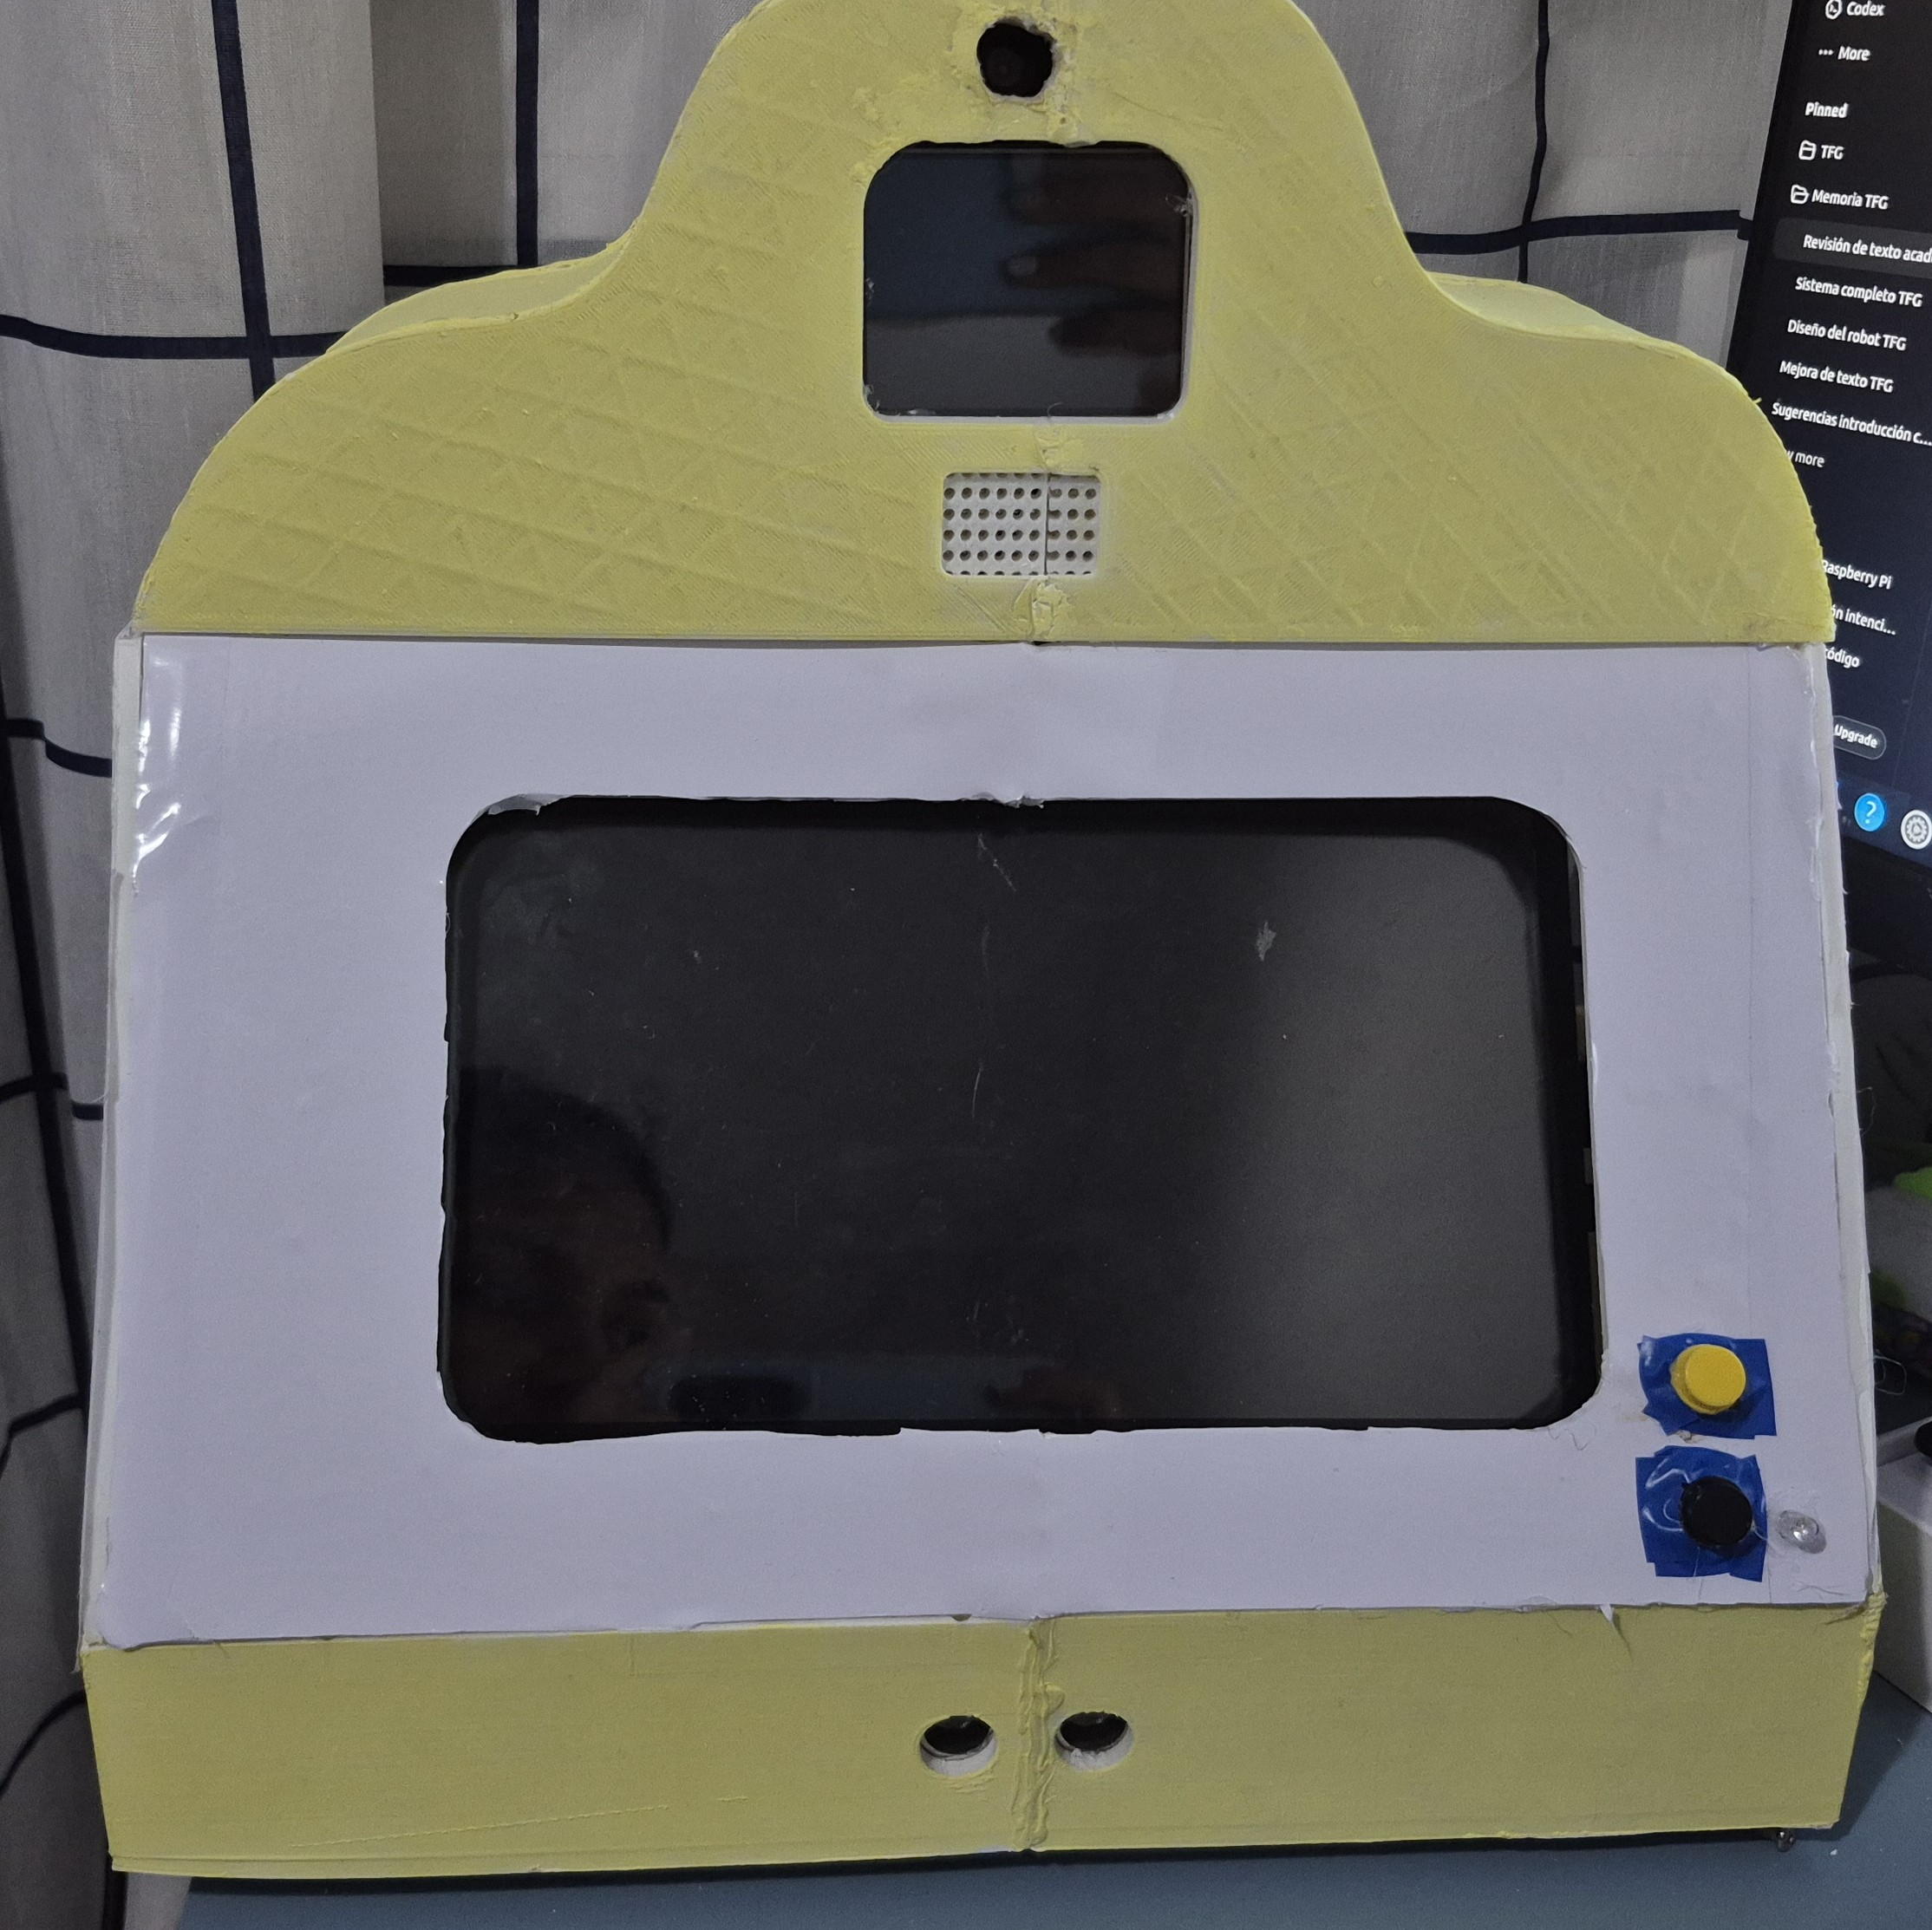
\includegraphics[width=0.36\textwidth]{figs/montaje1}
\hspace{0.03\textwidth}
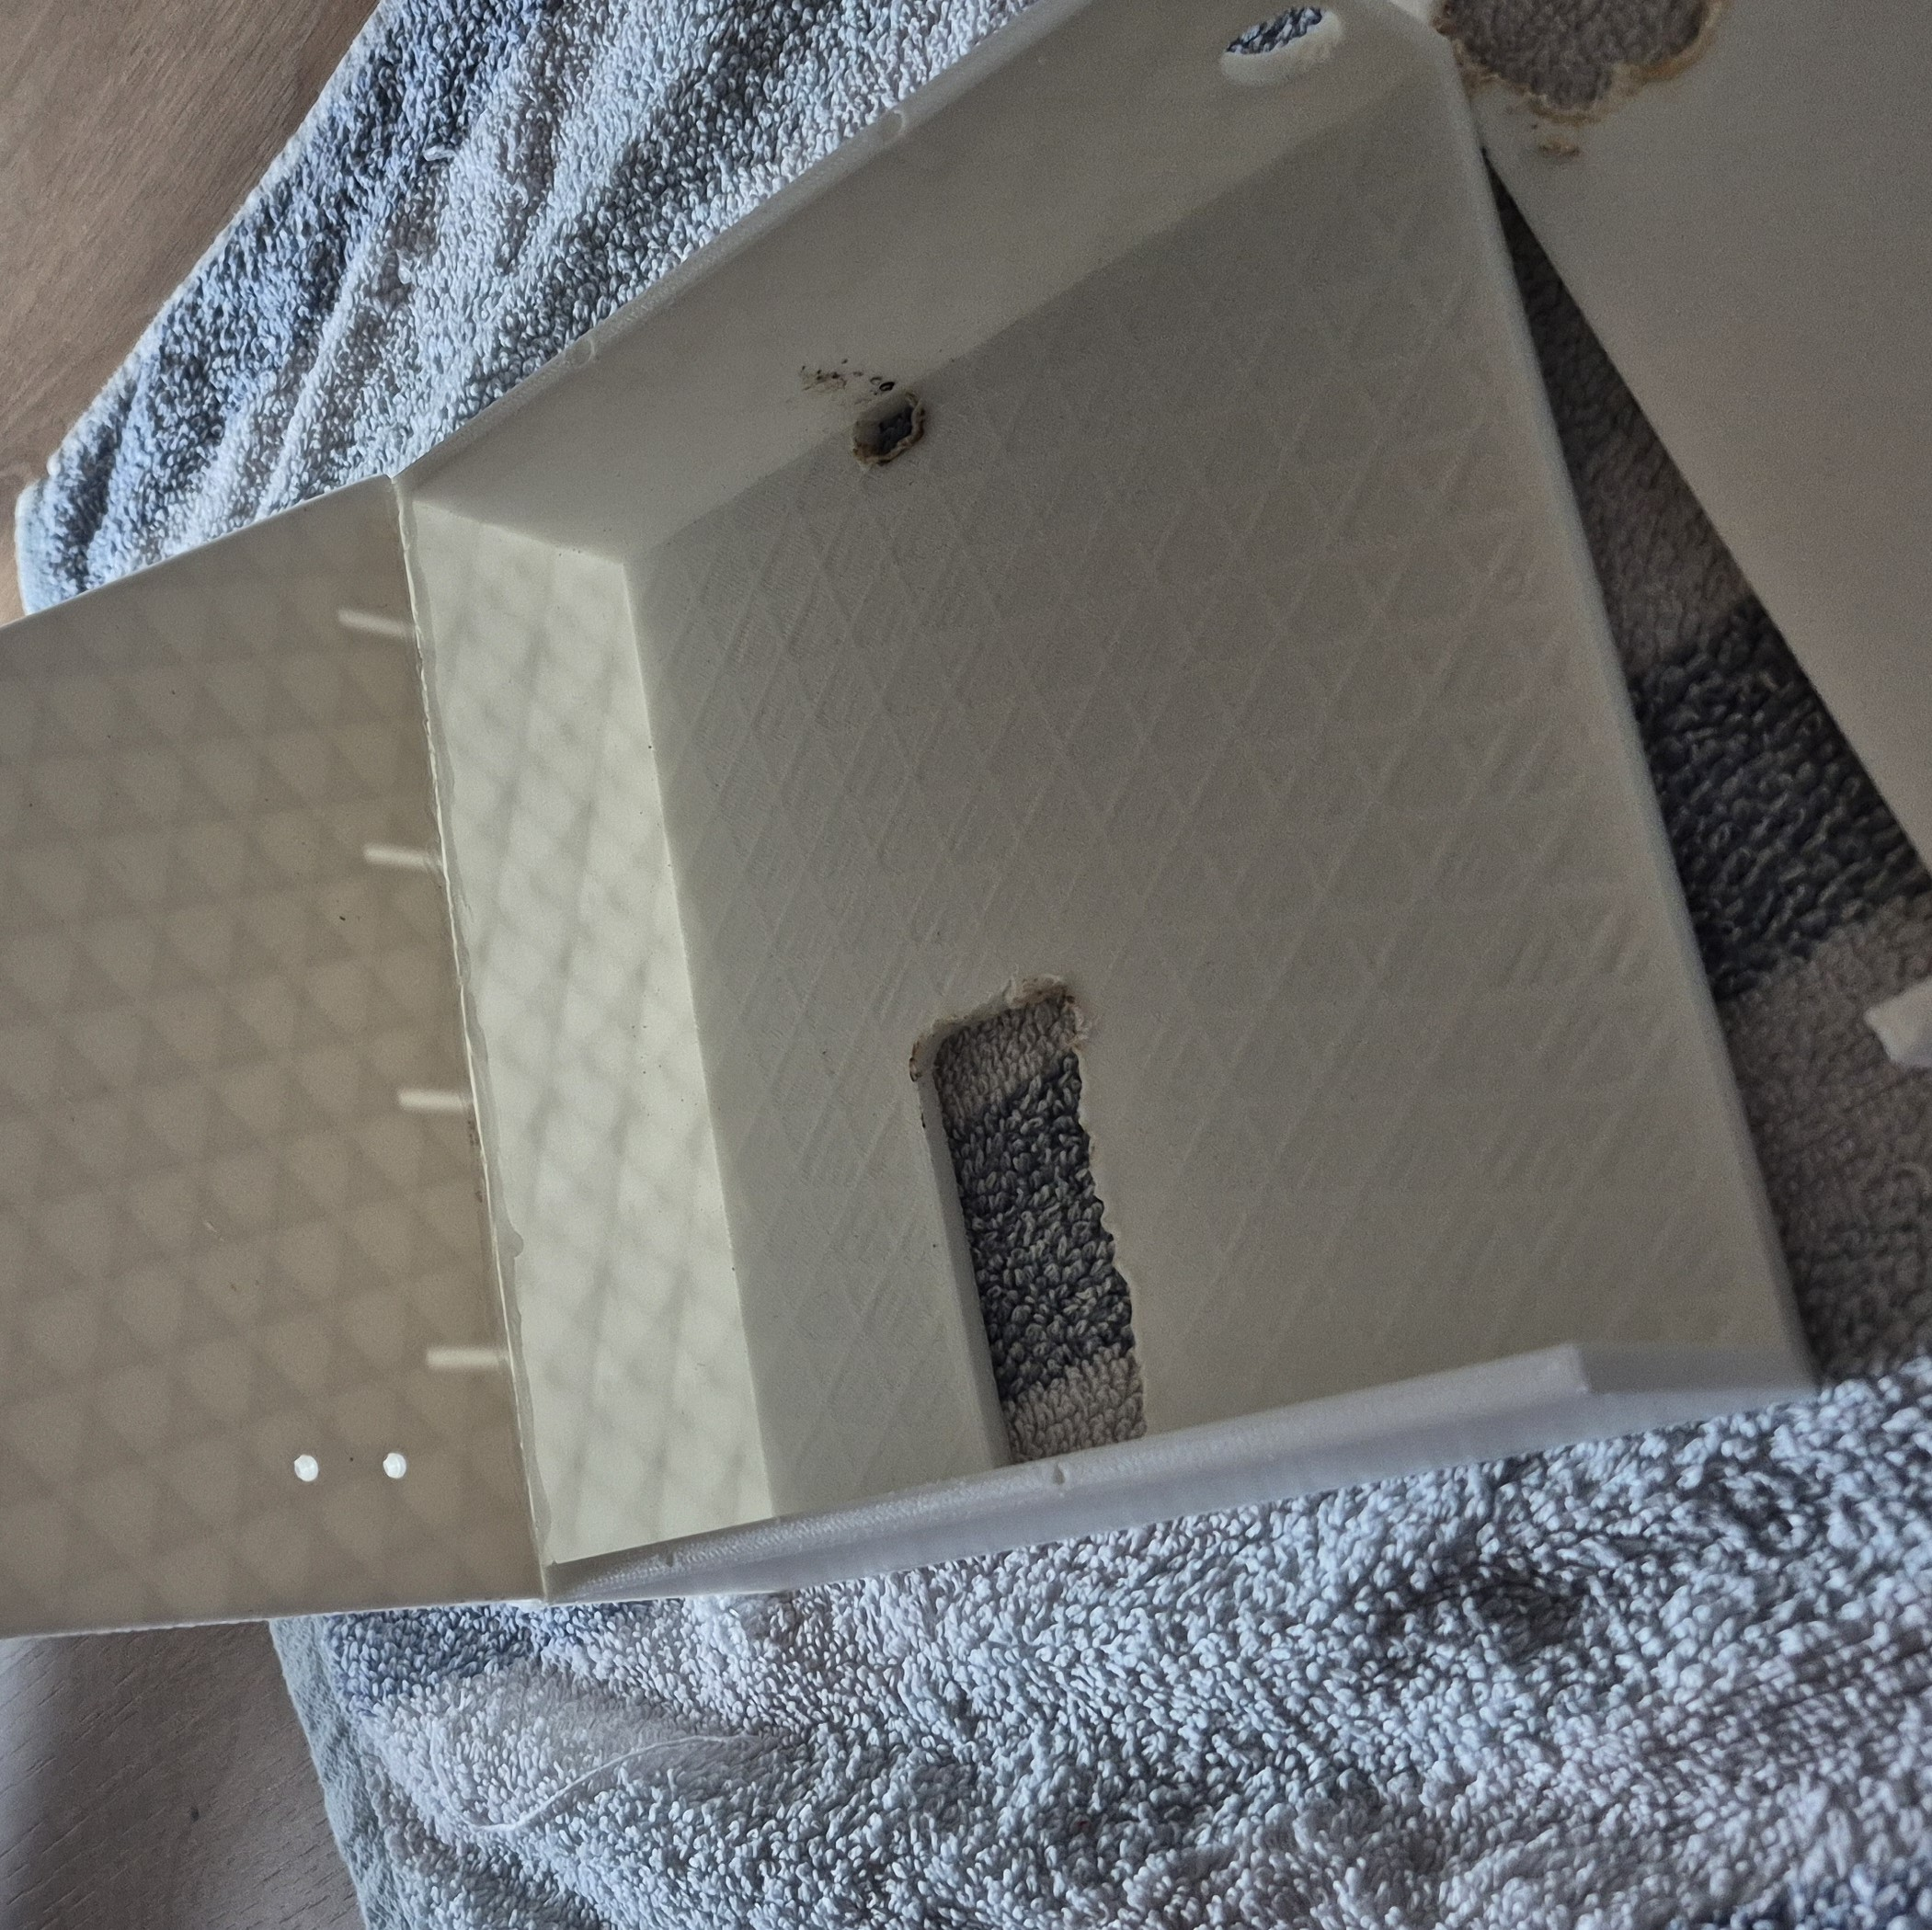
\includegraphics[width=0.36\textwidth]{figs/sol_p}

\vspace{0.4cm}

% Segunda fila
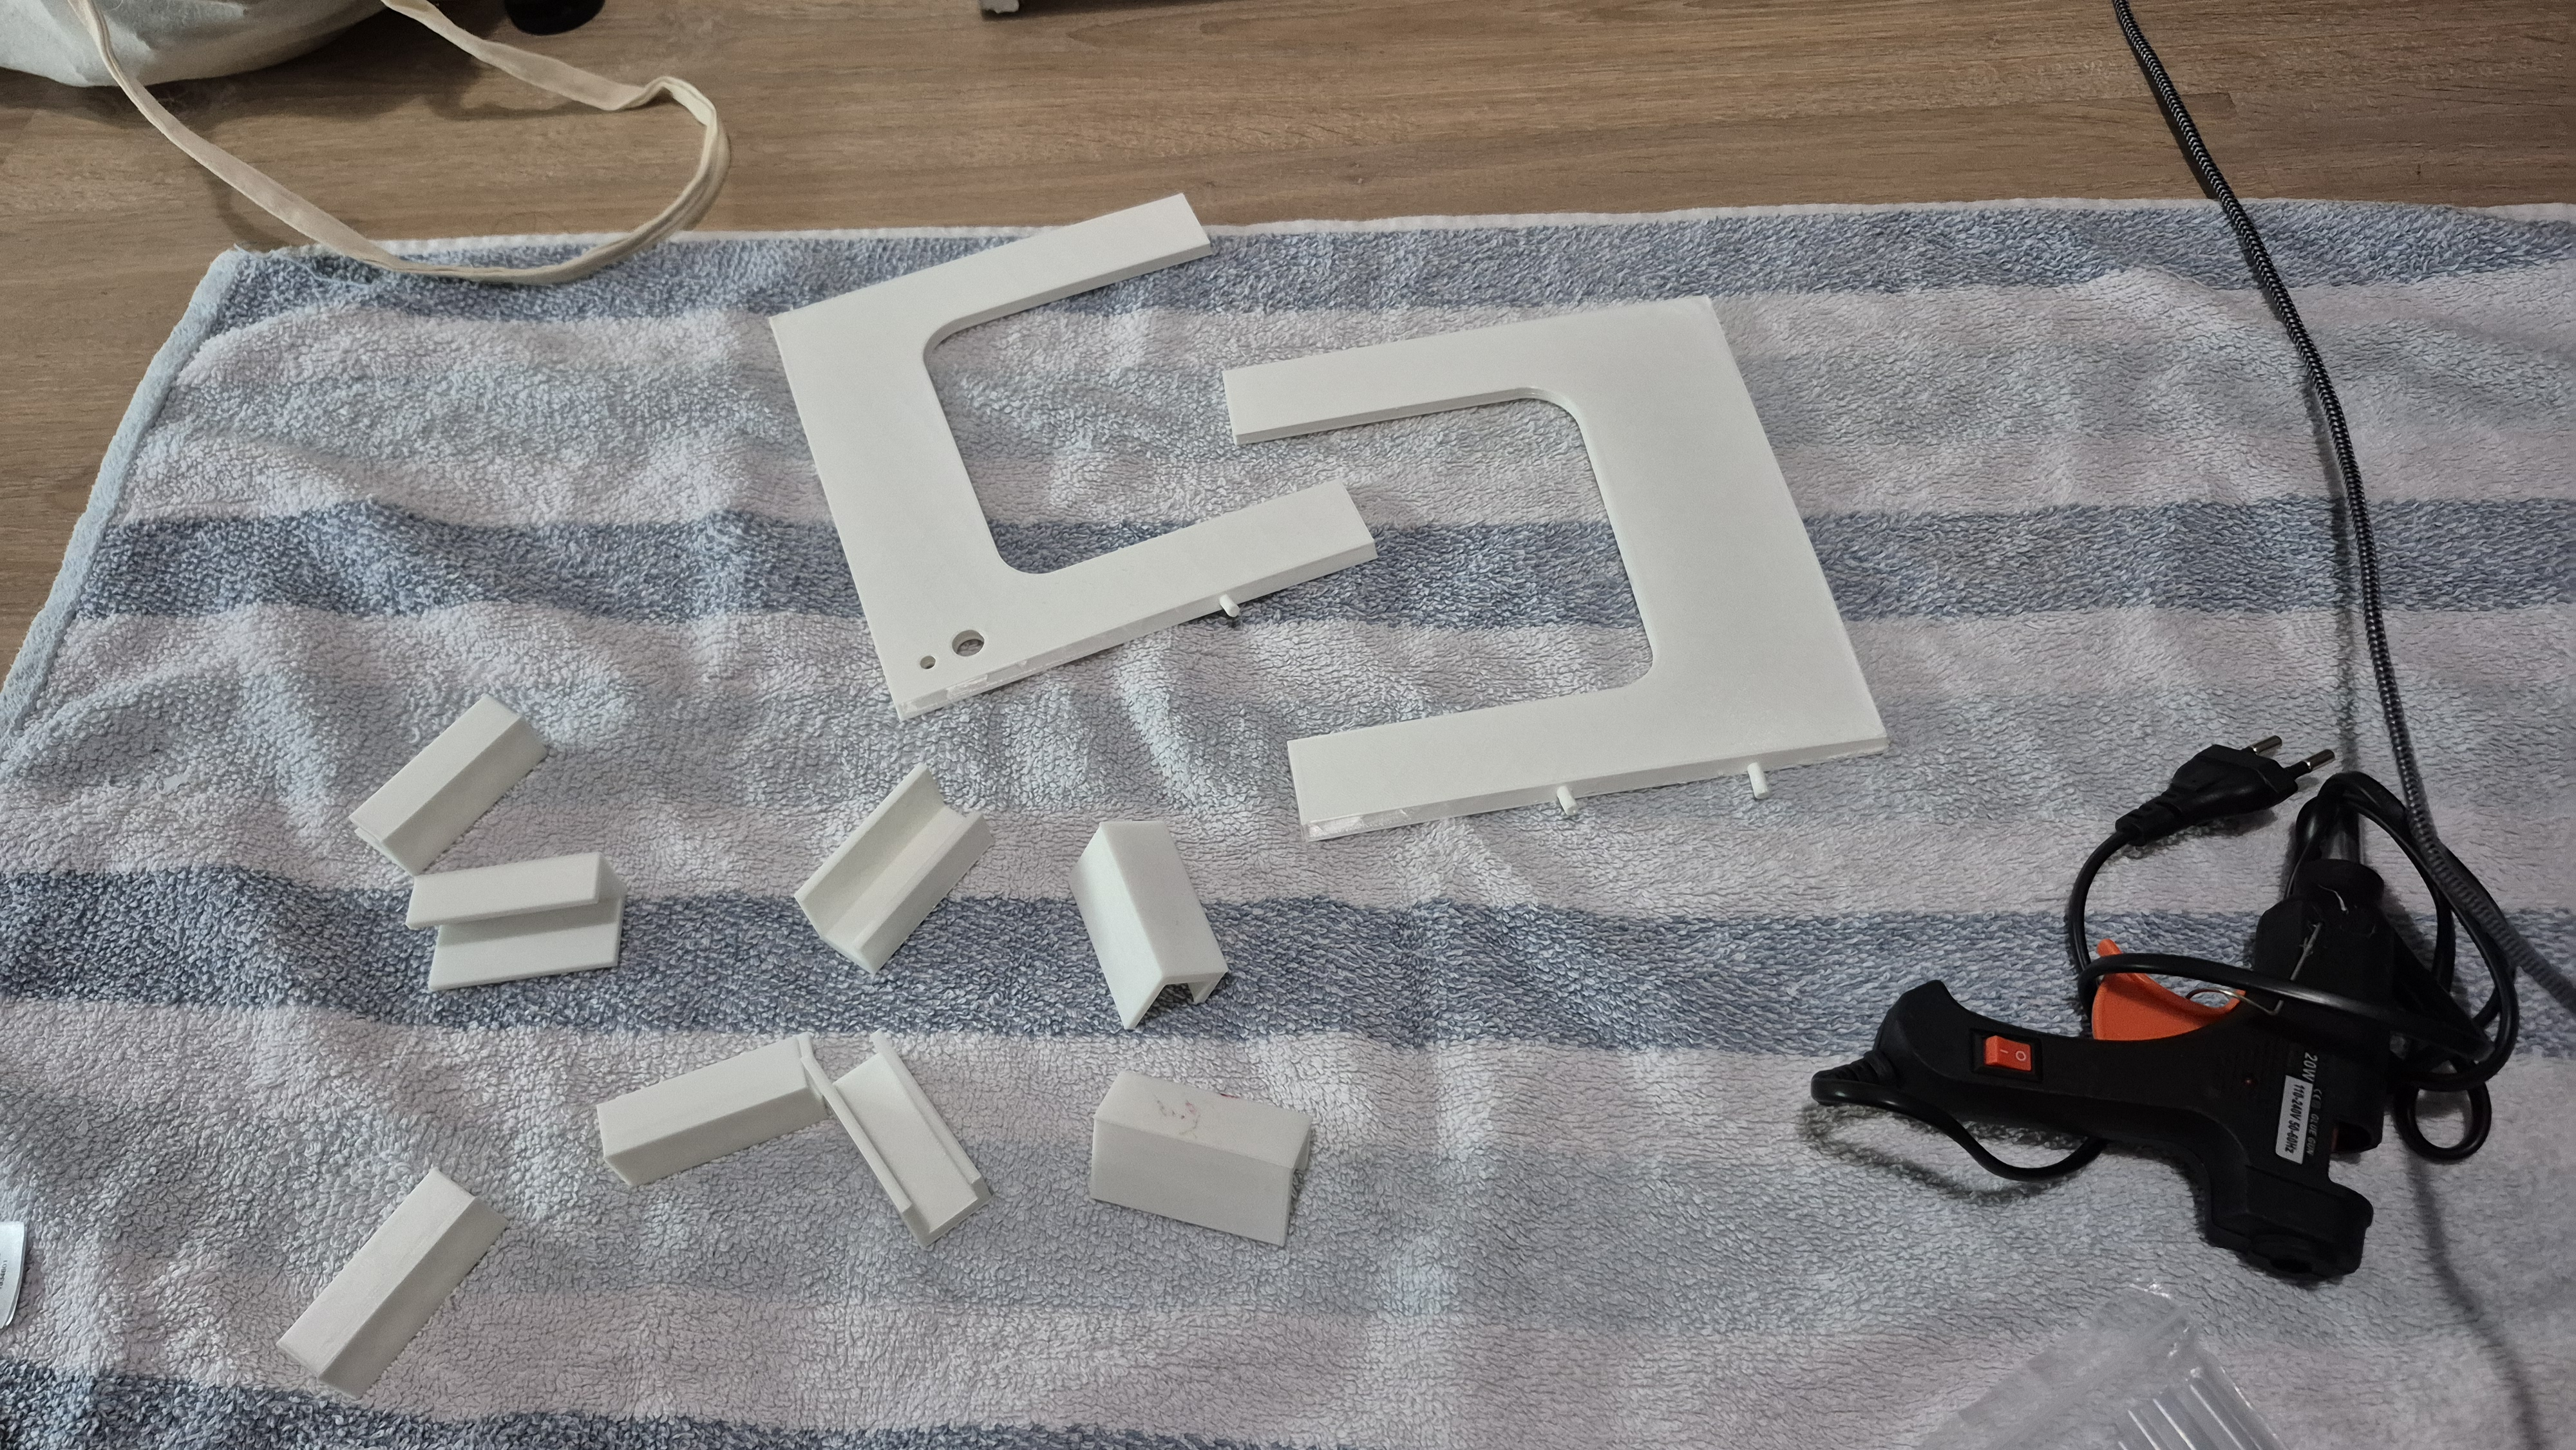
\includegraphics[width=0.38\textwidth]{figs/piezas}

\end{frame}



\begin{frame}
\frametitle{Reconocimiento facial}

\begin{figure}
\centering

\vspace{0.5cm}

\begin{tabular}{cc}
		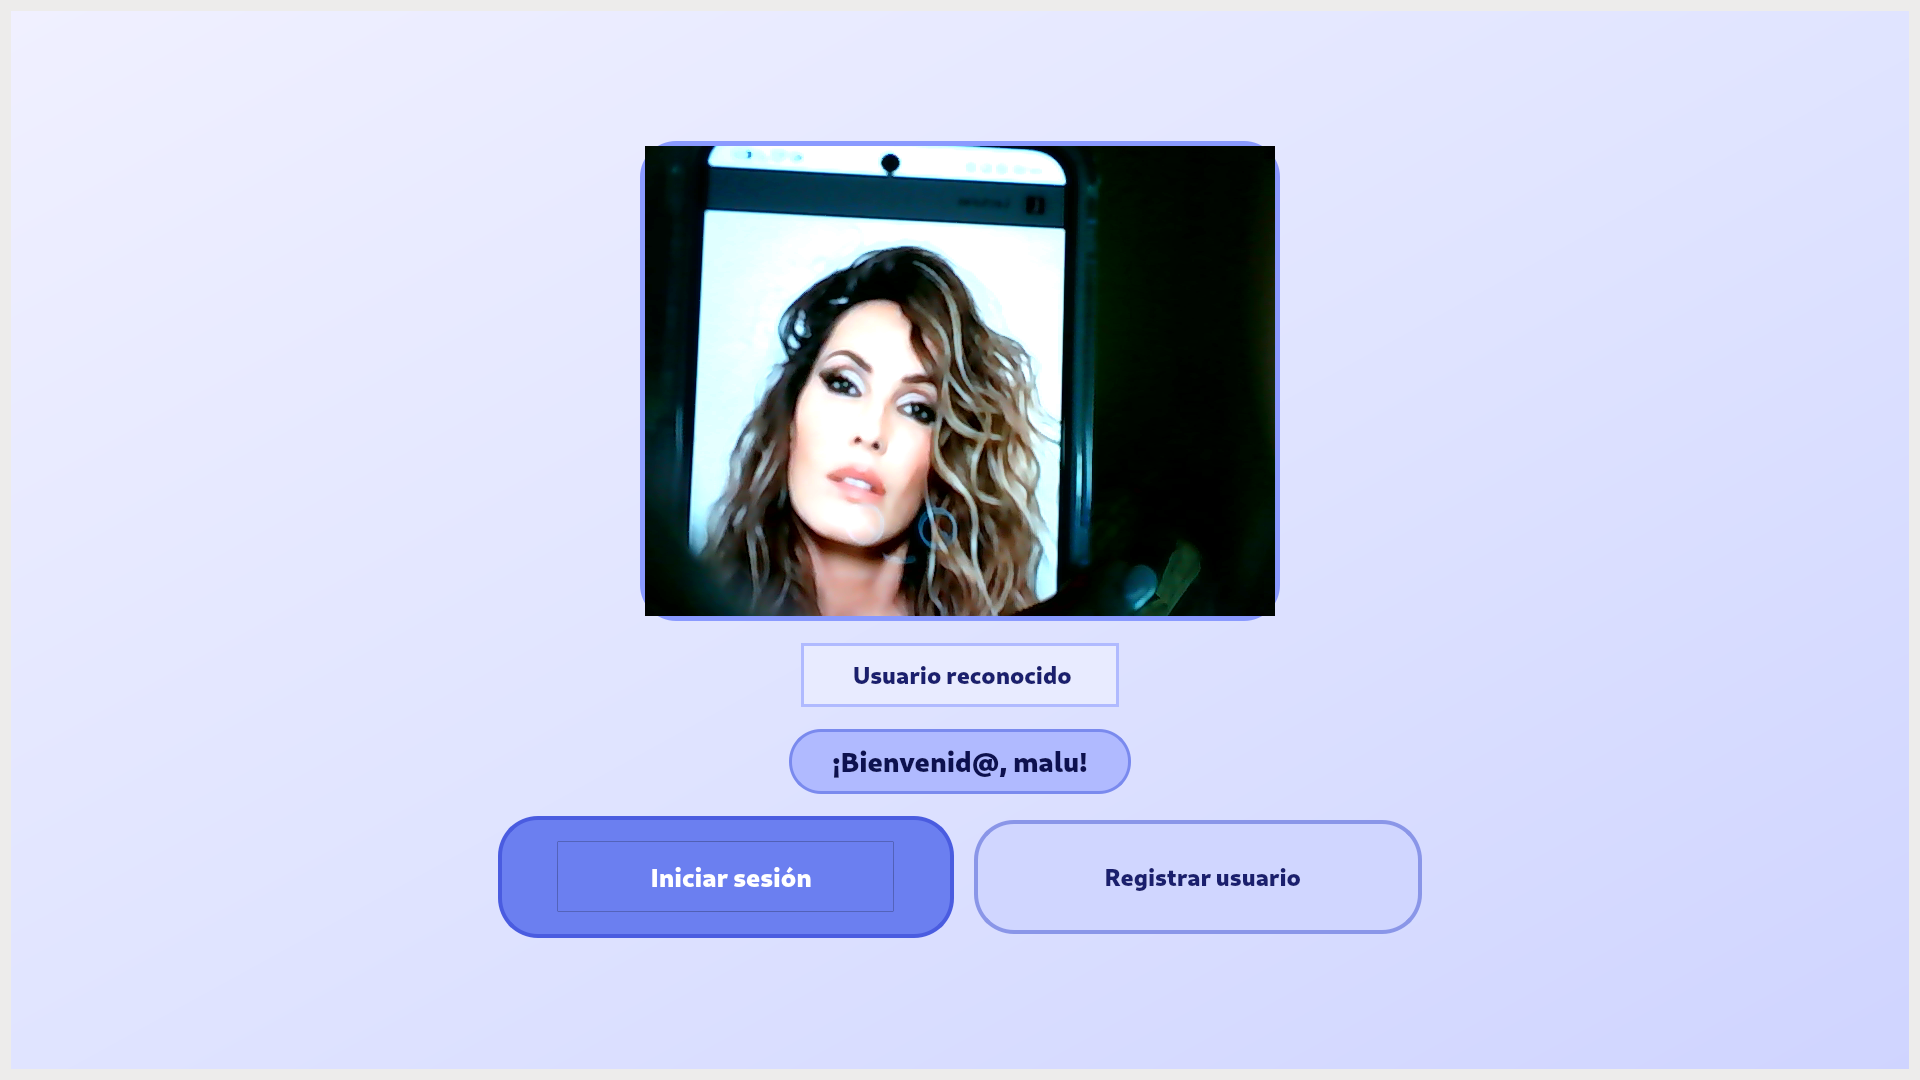
\includegraphics[width=0.3\textwidth, valign=m]{figs/logmal} & 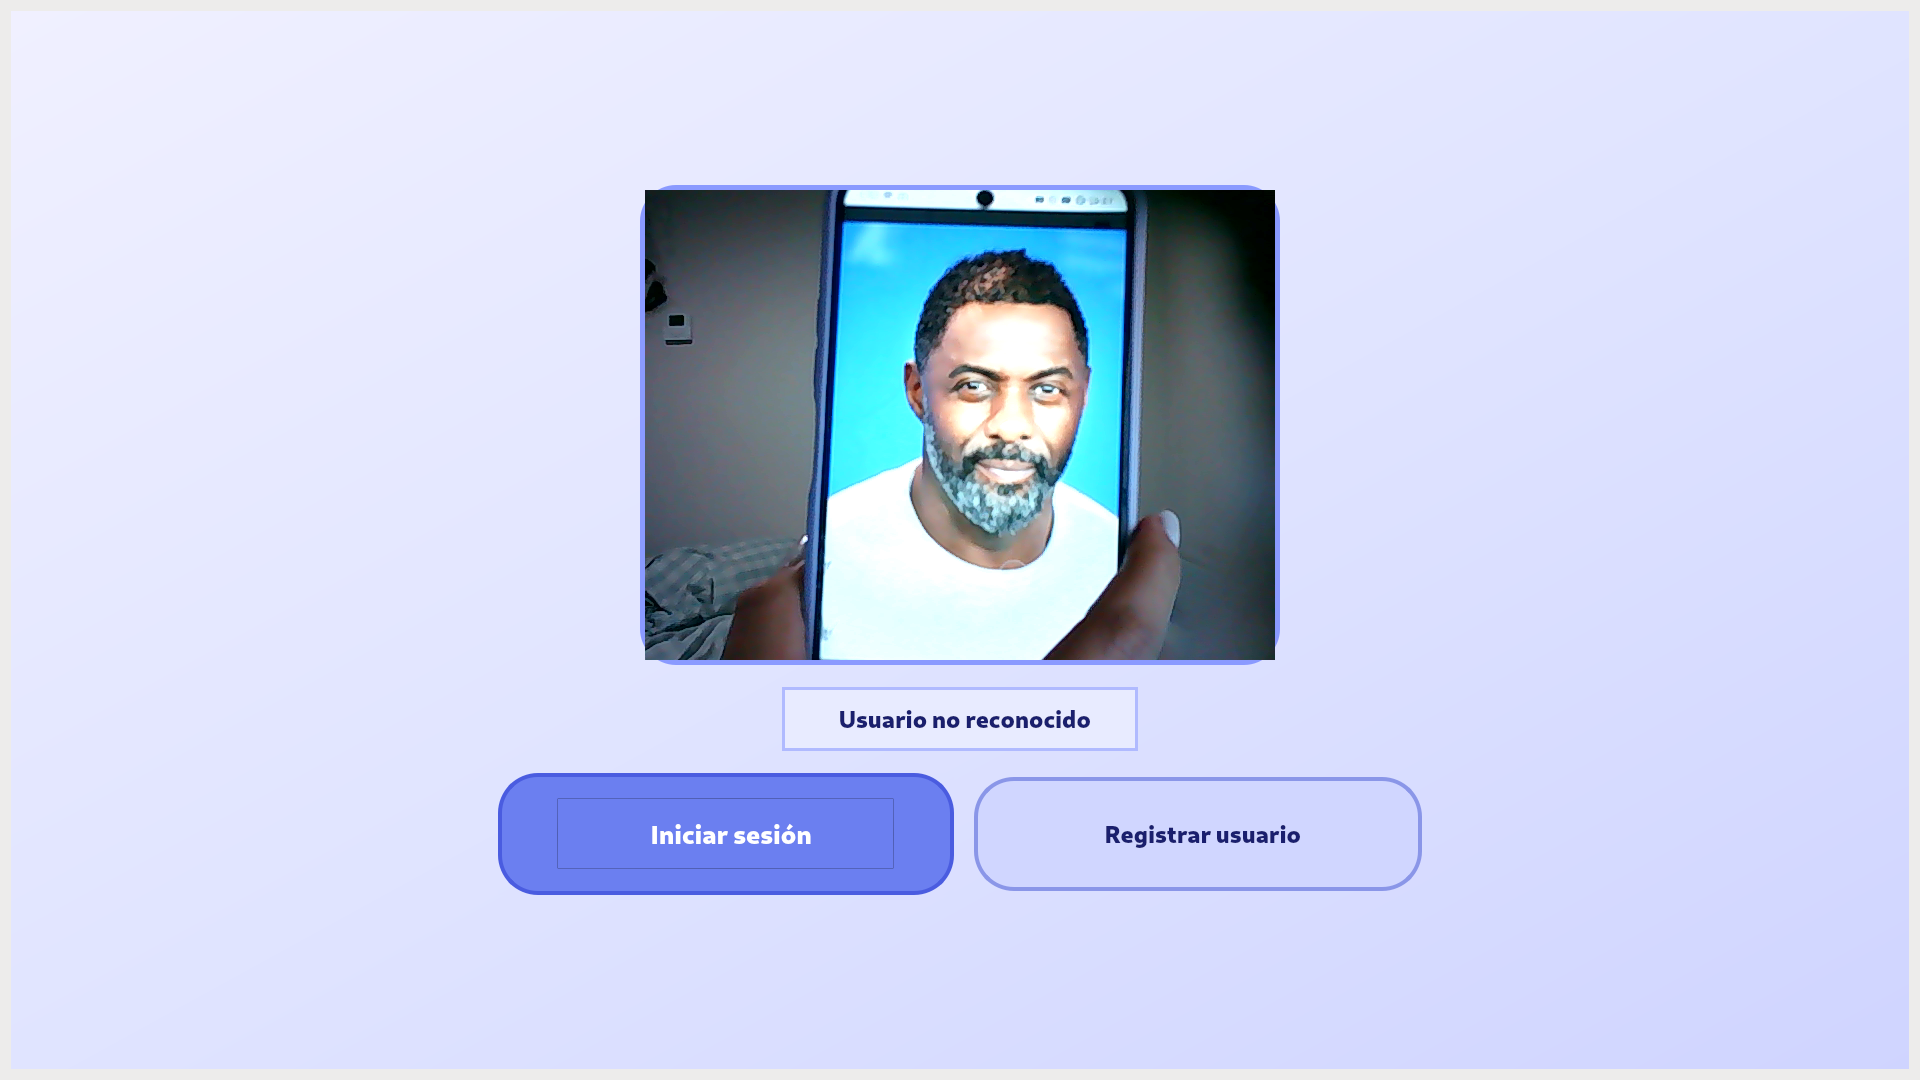
\includegraphics[width=0.3\textwidth, valign=m]{figs/idris} \\
		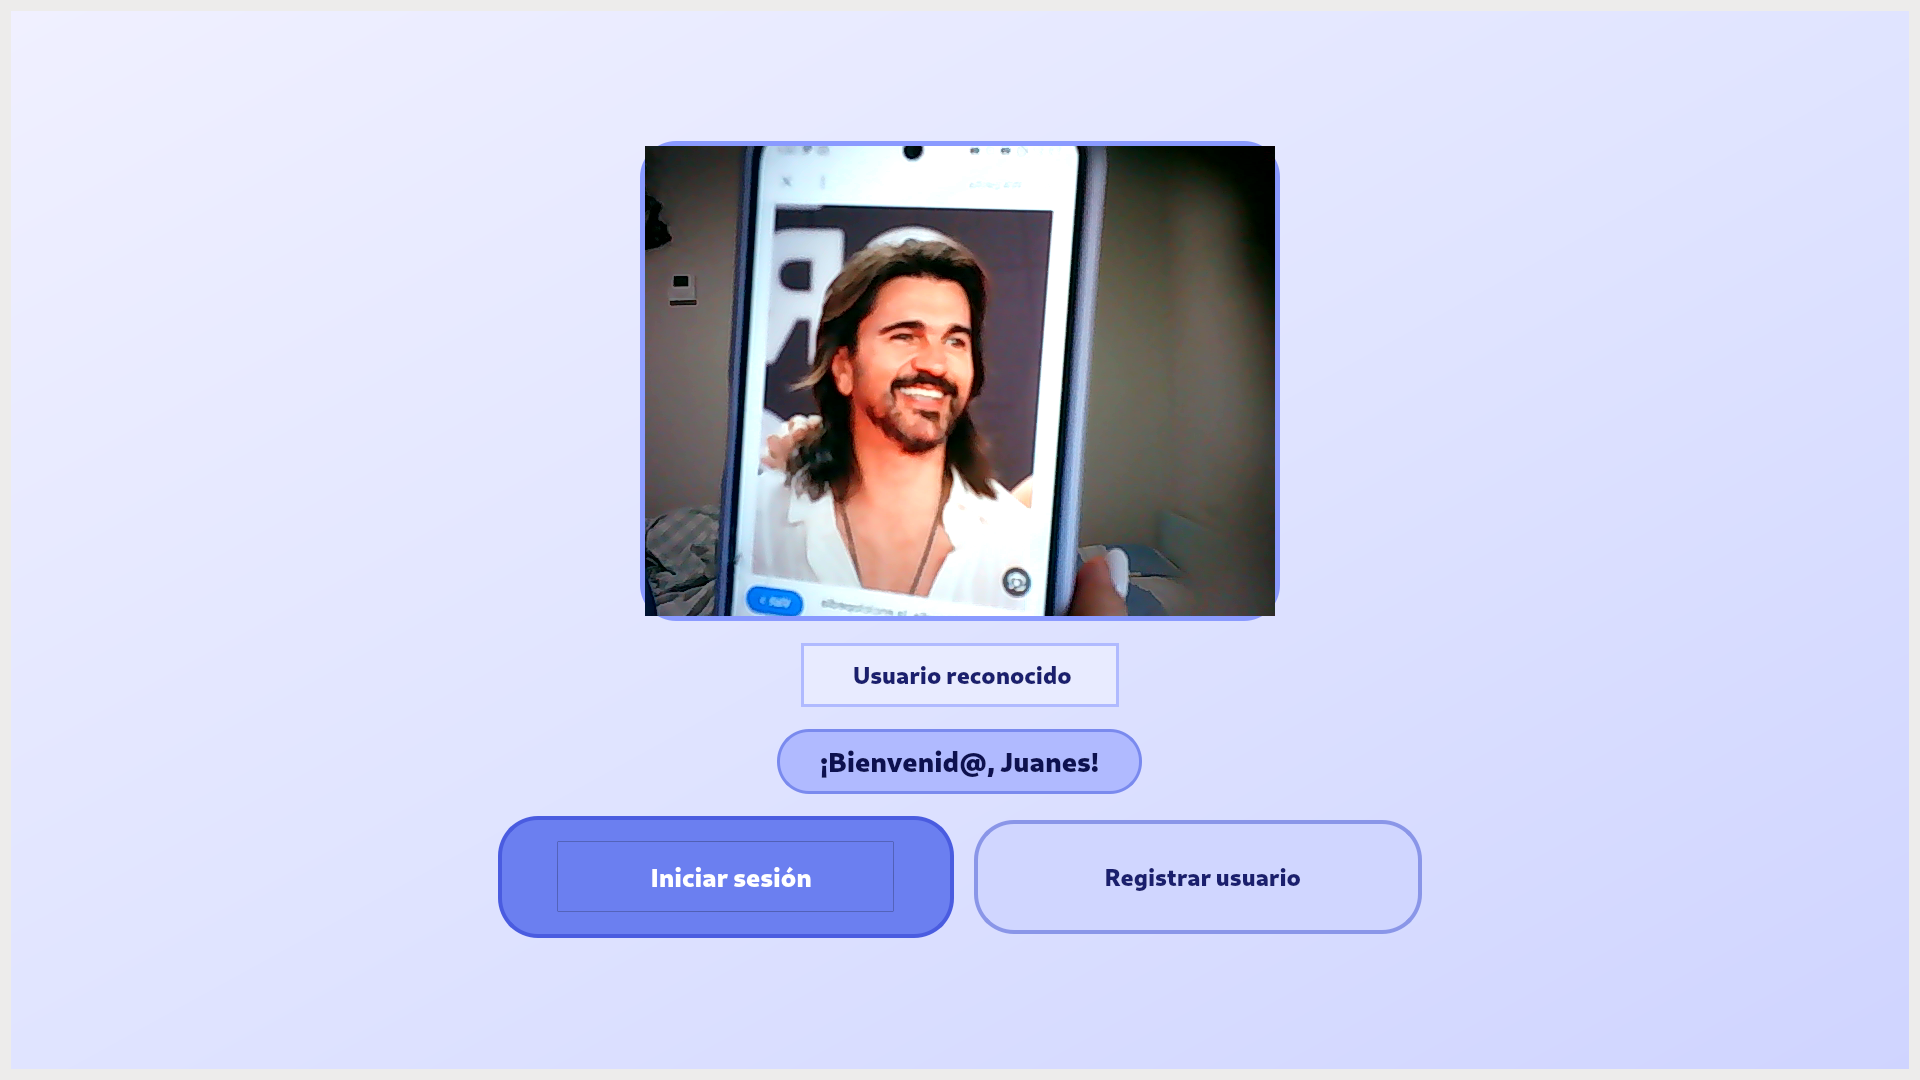
\includegraphics[width=0.3\textwidth, valign=m]{figs/juanes} & 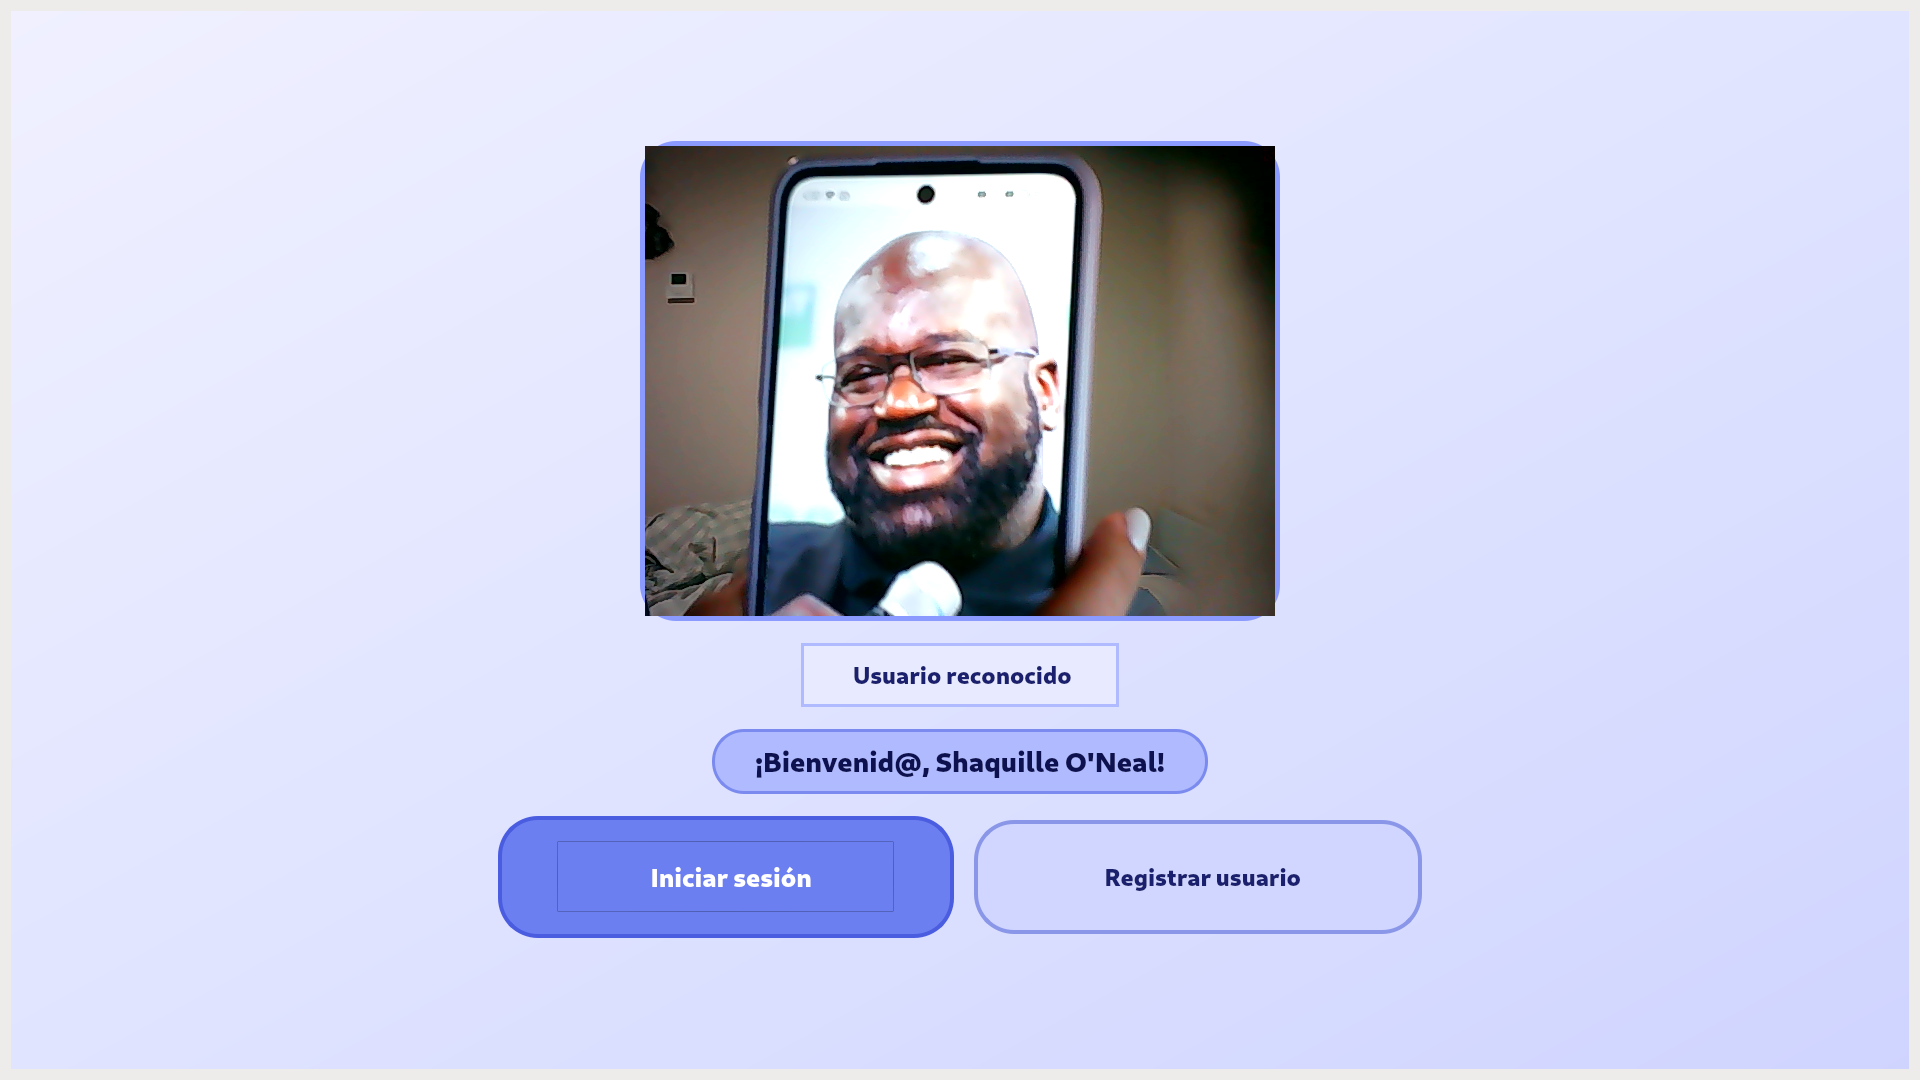
\includegraphics[width=0.3\textwidth, valign=m]{figs/sh}
\end{tabular}

\end{figure}

\end{frame}


\begin{frame}
\frametitle{Comparativa de modelos de lenguaje}
\centering

\begin{tabular}{|l|c|}
\hline
\textbf{Modelo} & \textbf{Latencia} \\
\hline
\textbf{\textcolor{green!60!black}{LLaMA 3 (Groq)}} & \textbf{\textcolor{green!60!black}{0.7--2.5 s}} \\
GPT-4 (Azure) & 4--9 s \\
Gemini & 3--60 s \\
\hline
\end{tabular}

\vspace{0.5cm}

\alert{LLaMA 3 fue el modelo seleccionado por ofrecer la menor latencia y un comportamiento más estable.}

\end{frame}


\section*{}
\begin{frame}{}
  \centering \Huge
  \emph{Conclusiones}
\note[item]{Para acabar esta presentación, vamos a repasar lo hecho, unas breves conclusiones y las líneas futuras.}
\end{frame}

\section{Conclusiones}


\begin{frame}
\begin{block}{Objetivos cumplidos}
\begin{itemize}

\note[item]{Para acabar esta presentación, vamos a repasar lo hecho, unas breves conclusiones y las líneas futuras.}

\item \alert{Robot asistencial} diseñado y fabricado.
\item Sistema  \alert{funcional} e \alert{integrado}.
\item Autenticación facial e IA conversacional.
\item Juegos para estimulación cognitiva.
\item Validación de las tecnologías empleadas.
\end{itemize}
\end{block}


\begin{block}{Líneas futuras}
\begin{itemize}
\note[item]{(Mejoras): (seguimiento del usuario y reconocimiento de emociones)}
\item Incorporar modelos de \alert{IA} más \alert{avanzados}.
\item Mejorar la interfaz y la experiencia de usuario.
\item Integrar todo el procesamiento en un \alert{único hardware}.
\item \alert{Ampliar las funcionalidades}.
\end{itemize}
\end{block}
\end{frame}

\begin{frame}[plain]
\large{\titlepage}
\note[item]{Y hasta aquí mi exposición.}
\note[item]{Quedo a disposición del tribunal...}
\end{frame}

\end{document}
